% This is a general template file for the LaTeX package SVJour3
% for Springer journals. Original by Springer Heidelberg, 2010/09/16
%
% Use it as the basis for your article. Delete % signs as needed.
%
% This template includes a few options for different layouts and
% content for various journals. Please consult a previous issue of
% your journal as needed.
%
%
\documentclass[graybox,footinfo]{svmult}

\smartqed
% \usepackage{mathptmx}       % selects Times Roman as basic font
\usepackage{helvet}         % selects Helvetica as sans-serif font
\usepackage{courier}        % selects Courier as typewriter font
\usepackage{type1cm}        % activate if the above 3 fonts are
% not available on your system
\usepackage{graphicx}       % standard LaTeX graphics tool
% when including figure files
%\usepackage{newtxtext}
%\usepackage{newtxmath}
%\usepackage{txfonts}

% \documentclass{svjour3}                     % onecolumn (standard format)
%\documentclass[smallcondensed]{svjour3}     % onecolumn (ditto)
%\documentclass[smallextended]{svjour3}       % onecolumn (second format)
%\documentclass[twocolumn]{svjour3}          % twocolumn
%

% \vec is not showing arruw, so redefine
% \AtBeginDocument{\renewcommand{\vec}[1]{\overrightarrow{#1}}}

% This approach is better than the above
% remove the definition of \vec by svjour3
\let\vec\relax
% restore the original definition in fontmath.ltx
\DeclareMathAccent{\vec}{\mathord}{letters}{"7E}

\RequirePackage{amsmath}
\RequirePackage{fix-cm}

\smartqed  % flush right qed marks, e.g. at end of proof
%
\usepackage{graphicx}
\usepackage{amssymb}
% \usepackage{amsthm}

% \usepackage{natbib}
\usepackage{xspace}
\usepackage{mathrsfs}  
\usepackage{hhline}
\usepackage{siunitx}
\usepackage{bbm}


%
% insert here the call for the packages your document requires
%\usepackage{mathptmx}      % use Times fonts if available on your TeX system
%\usepackage{latexsym}
% etc.
%
% Jag's 
\usepackage{tabu}
\usepackage{cancel}
\usepackage{algorithm}
\usepackage{algorithmicx}
\usepackage{algpseudocode}
%\usepackage[style=base]{caption}
%\usepackage[caption=false]{subfig}
%\usepackage{subcaption}
\usepackage{booktabs, mathtools}
%\usepackage[dvipsnames]{xcolor}
\usepackage{url}
\usepackage[titletoc,title]{appendix}
%\usepackage{refcheck}  % points out unused labels, refs ...

%\captionsetup{compatibility=false}

\algdef{SE}[DOWHILE]{Do}{doWhile}{\algorithmicdo}[1]{\algorithmicwhile\ #1}%

\DeclareMathOperator{\Order}{{\mathcal O}}

% please place your own definitions here and don't use \def but
% \newcommand{}{}
\newtheorem{prop}{Proposition}
\newtheorem{defn}{Definition}
\providecommand{\HickernellFJ}{Hickernell\xspace}
\newcommand{\bm}[1]{\boldsymbol{#1}}
\newcommand{\mSigma}{\mathsf{\Sigma}}
\newcommand{\mB}{\mathsf{B}}
\newcommand{\smallocite}[1]{{\small\ocite{#1}}}
\newcommand{\dif}[1]{\text{d}{#1}}
% \newcommand{\D}[1]{\text{d}{#1}}
\newcommand{\trace}[1]{\textup{trace}{#1}}

\newcommand{\naturals}{\mathbb{N}}
\newcommand{\natzero}{\mathbb{N}_0}
\newcommand{\reals}{\mathbb{R}}
\newcommand{\integers}{\mathbb{Z}}
\newcommand{\posIntegers}{\mathbb{Z}_{> 0}}
\newcommand{\complex}{\mathbb{C}}
\newcommand{\hilbert}{\mathbb{H}}
\newcommand{\Ex}{\mathbb{E}}
\newcommand{\bbone}{\mathbbm{1}}

\newcommand{\cf}{\mathcal{F}}
\newcommand{\cl}{\mathcal{L}}
\newcommand{\bbcl}{\bar{\boldsymbol{\cl}}}
\newcommand{\hbcl}{\hat{\boldsymbol{\cl}}}
\newcommand{\cx}{\mathcal{X}}
\newcommand{\tcx}{\widetilde{\cx}}
\newcommand{\rC}{\mathring{C}}
\newcommand{\ry}{\mathring{y}}
\newcommand{\rlambda}{\mathring{\lambda}}

\newcommand{\valpha}{{\bm{\alpha}}}
\newcommand{\vbeta}{{\bm{\beta}}}
\newcommand{\vDelta}{{\boldsymbol{\Delta}}}
\newcommand{\veta}{{\bm{\eta}}}
\newcommand{\vlambda}{{\bm{\lambda}}}
\newcommand{\vphi}{{\bm{\phi}}}
\newcommand{\vpsi}{{\bm{\psi}}}
\newcommand{\vtheta}{{\bm{\theta}}}
\newcommand{\vzeta}{{\bm{\zeta}}}
\newcommand{\vthetaMLE}{\bm{\theta}_{\MLE}}
\newcommand{\hvtheta}{\hat{\vtheta}}
\newcommand{\va}{\bm{a}}
\newcommand{\vA}{\bm{A}}
\newcommand{\vb}{\bm{b}}
\newcommand{\vc}{\bm{c}}
\newcommand{\vC}{\bm{C}}
\newcommand{\tvc}{\tilde{\bm{c}}}
\newcommand{\vg}{\bm{g}}
\newcommand{\vh}{\bm{h}}
\newcommand{\vf}{\bm{f}}
\newcommand{\vk}{\bm{k}}
\newcommand{\vl}{\bm{l}}
\newcommand{\vm}{\bm{m}}
\newcommand{\vs}{\bm{s}}
\newcommand{\vt}{\bm{t}}
\newcommand{\vv}{\bm{v}}
\newcommand{\vV}{\bm{V}}
\newcommand{\vw}{\bm{w}}
\newcommand{\vW}{\bm{W}}
\newcommand{\vx}{\bm{x}}
\newcommand{\dx}{\dif{{x}}}
\newcommand{\dt}{\dif{{t}}}
\newcommand{\dvx}{\dif{\bm{x}}}
\newcommand{\dvs}{\dif{\bm{s}}}
\newcommand{\dvt}{\dif{\bm{t}}}
\newcommand{\vrho}{\bm{\rho}}
\newcommand{\hy}{\hat{y}}
\newcommand{\vy}{\bm{y}}
\newcommand{\vY}{\bm{Y}}
\newcommand{\hvy}{\hat{\vy}}
\newcommand{\vz}{\bm{z}}
\newcommand{\vZ}{\bm{Z}}
\newcommand{\dvz}{\dif{\bm{z}}}
\newcommand{\tf}{\tilde{f}}
\newcommand{\vPsi}{\boldsymbol{\Psi}}

\newcommand{\fC}{\mathfrak{C}}
\newcommand{\hfC}{\mathring{\fC}}
\newcommand{\hbfC}{\mathring{\boldsymbol{\fC}}}
\newcommand{\fc}{\mathfrak{c}}
\newcommand{\bfc}{\boldsymbol{\mathfrak{c}}}

\newcommand{\tvv}{\tilde{\vv}}
\newcommand{\tvz}{\tilde{\vz}}

\newcommand{\vCvtheta}{{C_\vtheta}}
\newcommand{\hc}{\widehat{c}}

\newcommand{\hatvy}{\hat{\bm{y}}}
\newcommand{\haty}{\hat{y}}
\newcommand{\tvy}{\widetilde{\bm{y}}}
\newcommand{\ty}{\widetilde{y}}
\newcommand{\vzero}{\bm{0}}
\newcommand{\vone}{\bm{1}}
\newcommand{\tvone}{\tilde{\bm{1}}}
\newcommand{\mA}{\mathsf{A}}
\newcommand{\mC}{\mathsf{C}}
\newcommand{\mP}{\mathsf{P}}
\newcommand{\mK}{\mathsf{K}}
\newcommand{\rmC}{\mathring{\mathsf{C}}}
\newcommand{\mCtheta}{{\mathsf{C}_{\vtheta}}}
\newcommand{\mCthetaInv}{{\mathsf{C}^{-1}_{\vtheta}}}
%\newcommand{\mCthetaMLE}{{\mathsf{C}_{\vthetaMLE}}}
%\newcommand{\mCthetaInvMLE}{{\mathsf{C}^{-1}_{\vthetaMLE}}}
\newcommand{\mCInv}{\mathsf{C}^{-1}}
\newcommand{\cov}{{\textup{cov}}}
\newcommand{\var}{{\textup{var}}}
\newcommand{\opt}{{\textup{opt}}}


\newcommand{\tmC}{\widetilde{\mathsf{C}}}
\newcommand{\tlambda}{\tilde{\lambda}}

\newcommand{\mL}{\mathsf{L}}

\newcommand{\mLambda}{\mathsf{\Lambda}}
\newcommand{\mLambdaInv}{\mathsf{\Lambda}^{-1}}

\newcommand{\mG}{\mathsf{G}}
\newcommand{\mH}{\mathsf{H}}
\newcommand{\mV}{\mathsf{V}}
\newcommand{\mW}{\mathsf{W}}

\newcommand{\calN}{\mathcal{N}}
\newcommand{\me}{\mathrm{e}}

\newcommand{\tvrho}{\widetilde{\vrho}}
\newcommand{\heta}{\hat{\eta}}
\newcommand{\hmu}{\widehat{\mu}}
\newcommand{\hsigma}{\widehat{\sigma}}
\newcommand{\hnu}{\hat{\nu}}
\newcommand{\rhoCond}{\mathring{\vrho}}

\newcommand{\MVN}{\textup{MVN}}
\newcommand{\MLE}{\textup{EB}}
\newcommand{\full}{\textup{full}}
\newcommand{\GCV}{\textup{GCV}}


\newcommand{\wal}{\textup{wal}}
\newcommand{\CI}{\textup{CI}}
\newcommand{\NICE}{\textup{smth}}
\newcommand{\PEAKY}{\textup{pky}}
\newcommand{\NOISE}{\textup{noise}}
\newcommand{\TRUE}{\textup{true}}

%\newcommand{\errtol}{\text{tol}}
\newcommand{\errtol}{\varepsilon}
\newcommand{\errn}{\text{err}_{n}}
\newcommand{\diag}{\text{diag}}
\newcommand{\err}{\textup{err}}
\newcommand{\code}[1]{\texttt{#1}}

\def\abs#1{\ensuremath{\left \lvert #1 \right \rvert}}
\newcommand{\norm}[2][{}]{\ensuremath{\left \lVert #2 \right \rVert}_{#1}}
\newcommand{\ip}[3][{}]{\ensuremath{\left \langle #2, #3 \right \rangle_{#1}}}

\DeclarePairedDelimiter{\ceil}{\lceil}{\rceil}

\newenvironment{nalign}{
    \begin{equation}
    \begin{aligned}
}{
    \end{aligned}
    \end{equation}
    \ignorespacesafterend
}

\providecommand{\argmin}{\operatorname*{argmin}}
\providecommand{\argmax}{\operatorname*{argmax}}
\newcommand\figref{Figure~\ref}
\newcommand\secref{Section~\ref}

\graphicspath{{.}{./figures/grey/}{D:/Mega/MyWriteupBackup/Sep_2ndweek_1/}}
%\graphicspath{{./figures/}}

%
% Insert the name of "your journal" with
% \journalname{Automatic Bayesian Cubature}
%

\newcommand{\FJHNote}[1]{{\textcolor{blue}{FJH: #1}}}
\newcommand{\JRNote}[1]{{\textcolor{green}{JR: #1}}}


\allowdisplaybreaks
\begin{document}
\setlength\abovedisplayskip{1pt}
\setlength{\belowdisplayskip}{1pt}

\title{Fast Automatic Bayesian Cubature Using Sobol' Sampling
%\thanks{}
}
% Grants or other notes about the article that should go on the front
% page should be placed within the \thanks{} command in the title
% (and the %-sign in front of \thanks{} should be deleted)
%
% General acknowledgments should be placed at the end of the article.

%\subtitle{Do you have a subtitle?\\ If so, write it here}

%\titlerunning{Short form of title}        % if too long for running head

\author{R. Jagadeeswaran         \and
        Fred J. Hickernell %etc.
}

%\authorrunning{Short form of author list} % if too long for running head

\institute{R. Jagadeeswaran \at
              Department of Applied Mathematics, \\
              Illinois Institute of Technology \\
              10 W. 32nd St., Room 220,
              Chicago IL 60616\\
              \email{jrathin1@iit.edu}           %  \\
%             \emph{Present address:} of F. Author  %  if needed
           \and
           Fred J. Hickernell \at
           Center for Interdisciplinary Scientific Computation and \\
           Department of Applied Mathematics \\
           Illinois Institute of Technology \\
           10 W. 32nd St., Room 220, 
           Chicago IL 60616
           \\
           \email{hickernell@iit.edu} 
}

\date{Received: date / Accepted: date}
% The correct dates will be entered by the editor

\maketitle

\abstract{
	Automatic cubatures approximate integrals to user-specified error tolerances.  For high dimensional problems, it is difficult to adaptively change the sampling pattern, but one can automatically determine the sample size, $n$, given a reasonable, fixed sampling pattern. This approach is pursued in \cite{RatHic19a}, where a Bayesian perspective is used to construct a credible interval for the integral, and the computation is terminated when the half-widths of the interval is no greater than the required error tolerance.  In \cite{RatHic19a} integration lattice sampling is employed and the computations are expedited by the use of a fast Fourier transform because the covariance kernels for the Gaussian process prior on the integrand are chosen to be shift-invariant.  In this chapter, we extend our fast automatic Bayesian cubature to digital net sampling via digital shift-invariant covariance kernels and fast Walsh transforms.
	Our algorithm is implemented in the Guaranteed Automatic Integration Library (GAIL).
}





\section{Introduction}
\label{intro}

Cubature, or numerical multivariate integration, is the problem of inferring a numerical value for a definite integral, 
\begin{equation}
\label{eqn:defn_mu}
\mu:= \mu(f) := \Ex[f(\boldsymbol{X})] = \int_{[0,1]^d} f(\vx)\, \dvx, 
\end{equation}
when no closed-form analytic expression exists. Typically, values of $f$ are accessible through a black-box function routine. ur goal is to construct a cubature, $\hmu = \hmu(f)$, depending only on integrand values at the nodes $\{\vx_i\}_{i=1}^n$, and determine the $n$ which satisfies the error criterion
\begin{equation}
\label{eqn:err_crit} 
\abs{\mu - \hmu} \leq \errtol
\end{equation}
with high probability. This article extends the fast Bayesian cubature ideas presented in \cite{RatHic19a} to digital sequences \cite{DicPil10a}.


Cubature is a key component of many problems in scientific computing, finance \cite{Gla03}, statistical modeling, imaging \cite{Keller2013}, uncertainty quantification, and machine learning \cite{Goodfellow-et-al-2016}. 
%\JRNote{add references}
The original form of the integral may require a suitable variable transformation to become \eqref{eqn:defn_mu}. This process is addressed in \cite{BecHae92b, Sid08a, Sid93, Lau96a, CriEtal07}. 

Following the Bayesian numerics approach of \cite{Dia88a}, \cite{OHa91a}, Rasmussen and Ghahramani~\cite{RasGha03a}, \cite{BriEtal18a}, and others, we assume that our integrand is an instance of a Gaussian process, $\mathcal{GP}(m,s^2 C_\vtheta)$, and construct a probabilistic error bound for $\mu$ to via a Bayesian credible interval.  The integrand is sampled until the credible interval becomes small enough to satisfy \eqref{eqn:err_crit} with high probability.  

Our approach to fast Bayesian cubature \cite{RatHic19a} emphasizes 
\begin{itemize}
    \item Choosing covariance kernels, $C_\vtheta:[0,1]^d \times [0,1]^d \to \reals$, for which the symmetric, positive definite Gram matrices, $\mC_\vtheta = \left(  C_\vtheta(\vx_i,\vx_j)  \right)_{i,j=1}^n$,
    have an eigenvalue-eigenvector decomposition of the form $\mC_\vtheta = \mV \mLambda_\vtheta \mV^H/n$, where
    \begin{subequations} \label{fastcompAssump}
	\begin{gather}
	\label{fastcompAssumpA}
	\mV \text{ may be identified analytically}, \\
	\label{fastcompAssumpB}
	\vv_1 = \vV_1 = \vone, \\
	\label{fastcompAssumpC}
	\text{ Computing $\mV^H \vb$ requires only $\Order(n \log n)$ operations } \forall \vb, \\
	\label{addAssump}
\int_{[0,1]^d} C_\vtheta(\vt,\vx) \, \D \vt = 1 \qquad \forall \vx \in [0,1]^d,
	\end{gather}
\end{subequations}
and
\item The hyperparameters of the Gaussian process, $m$, $s$, and $\vtheta$ are tuned to increase the likelihood that $f$ is a typical integrand $f$ and not an outlier.
\end{itemize}
Our earlier work, \cite{RatHic19a}, which laid the foundation for this approach, focused on lattice nodes and shift-invariant kernels. In that context the computation of $\mV^H \vb$ is a one-dimensional fast Fourier transform.  This chapter focuses on digital sequences, such as Sobol' sequences \cite{Sob67}, and covariance kernels that are digital shift-invariant.  In this case the computation of $\mV^H \vb$ is a fast Walsh-Hadamard transform. 


\iffalse 
We call the transformation $\vb \mapsto \mV^H \vb$ a \emph{fast Bayesian transform} and $C_\vtheta$ a \emph{fast Bayesian transform kernel} for the matching nodes $\{\vx_i\}_{i=1}^\infty$.  The covariance kernels used in practice also may satisfy an additional assumption:
\fi

The next section summarizes the key formulae from \cite{RatHic19a}.  Section \ref{sec:sobol_walsh} extends fast Bayesian cubature to digital nets and digital-shift invariant kernels defined in terms of Walsh functions.  Section \ref{sec:NumExp} presents numerical experiments that illustrate these ideas.  


%%%%%%%%%%%%%%%%%%%%%%%%%%%%%%%%%%%%%%%%%%%%%%%%%%%%%%%%%%%%%%%%%%%%%%%%%%%%%%%%%%%%%
%%%%%%%%%%%%%%%%%%%%%%%%%%%%%%%%%%%%%%%%%%%%%%%%%%%%%%%%%%%%%%%%%%%%%%%%%%%%%%%%%%%%%


\section{Bayesian Cubature}
\label{sec:BC} 

\subsection{Bayesian Posterior Error}
\label{sec:BayesPostErr}

We assume the integrand, $f$, is an instance of a real-valued stochastic Gaussian process, i.e., $f \sim \mathcal{GP}(m,s^2 C_\vtheta)$.  Specifically, $f$ is a random function with constant mean $m$ and covariance kernel $s^2C_\vtheta$, where $s$ is a positive scale factor, and $C_\vtheta: [0,1]^d \times [0,1]^d \to \mathbb{R} $ is a symmetric, positive-definite function and, parameterized by $\vtheta$:
\begin{multline} \label{FJH:eq:CondPosDef}
\mC_\vtheta^T = \mC_\vtheta,  \quad \va^T \mC_\vtheta \va > 0, \quad \text{where }  \mC_\vtheta = \left(  C_\vtheta(\vx_i,\vx_j)  \right)_{i,j=1}^n,\\
\text{for all } \va \ne 0, \;
n\in \mathbb{N}, \; \text{distinct} \; \vx_1, \ldots, \vx_n \in [0,1]^d.
\end{multline}

As shown in \cite{RatHic19a}, a credible interval for the integral is given in terms of the nodes, $\{\vx_i\}_{i=1}^n$, and the covariance kernel, $C_\vtheta$,  by 
\begin{subequations} \label{eqn_prob_confidence_interval}
	\begin{gather}
	\mathbb{P}_f \left[
	|\mu-\hmu| \leq \err_{\CI}
	\right] = 99\%, \\
	\err_{\CI} = 2.58 s \sqrt{c_{0,\vtheta} - \vc_\vtheta^T\mC_\vtheta^{-1}\vc_\vtheta}.
	\end{gather}
\end{subequations}
where
\begin{subequations} \label{eqn:fGaussDist}
\begin{gather}
\label{eqn:fGaussDist_c0}
	c_{0,\vtheta} := \int_{[0,1]^{d} \times [0,1]^{d}} C_\vtheta(\vx,\vt) \, \dif{\vx} \, \dif{\vt}, \\
	\label{eqn:fGaussDist_vc}
 \vc_\vtheta := \left(  \int_{[0,1]^d} C_\vtheta(\vt,\vx_i) \, \D \vt \right)_{i=1}^n.
	\end{gather}
\end{subequations}
Naturally, $2.58$ and $99\%$ can be replaced by other quantiles and credible levels.  The formula for $\hmu$ in terms of the function values at the nodes is given below in Section \ref{sec:hyperparameters}.

The credible interval in \eqref{eqn_prob_confidence_interval} suggests how our automatic Bayesian cubature proceeds.  Integrand data is accumulated until the width of the credible interval, $\err_{\CI}$, is no greater than the error tolerance.  As $n$ increases, one expects $c_{0,\vtheta} - \vc_\vtheta^T\mC_\vtheta^{-1}\vc_\vtheta$ to decrease for well-chosen nodes, $\{\vx_i\}_{i=1}^n$. 



\subsection{Fast Bayesian Transform Kernel}
\label{sec:fast_BC}

Normally, computing $\err_{\CI}$ in  \eqref{eqn_prob_confidence_interval} would require $\Order\bigl( n^3 \bigr)$ operations to perform the equivalent of a matrix inversion.  However, for a certain class of kernels, $C$, termed fast Bayesian transform kernels in \cite{RatHic19a}, this cost can be drastically reduced.  The key is for the covariance kernel to match the nodes.

Let the eigenvector-eigenvalue decomposition of the Gram matrix be expressed as follows:
\begin{align}
\nonumber
\mC = \mCtheta &= \Big(C_\vtheta(\vx_i,\vx_j)\Big)_{i,j=1}^n  = (\vC_{\vtheta,1},...,\vC_{\vtheta,n}) 
\\
\label{eqn:ftk_factor}
&= \frac 1n \mV \mLambda_\vtheta \mV^H , 
\quad \quad \mV^H = n \mV^{-1}, \\
\nonumber
\mV &= (\vv_1,...,\vv_n)^T = (\vV_1,...,\vV_n),
\end{align}
where $\mV^H$ is the Hermitian of $\mV$.
The columns of matrix $\mV$ are eigenvectors of $\mC_\vtheta$, and $\mLambda$ is a diagonal matrix of eigenvalues of $\mC_\vtheta$. The normalization of $\mV$ assumed in \eqref{eqn:ftk_factor} allows the first eigenvector, $\vV_1$, to be the vector of ones in \eqref{fastcompAssumpB} below.

We make three assumptions that allow the fast computation of $\widetilde{\vb} := \mV^H \vb$:
\begin{subequations} \label{fastcompAssump}
	\begin{gather}
	\label{fastcompAssumpA}
	\mV \text{ may be identified analytically}, \\
	\label{fastcompAssumpB}
	\vv_1 = \vV_1 = \vone, \\
	\label{fastcompAssumpC}
	\text{ Computing $\mV^H \vb$ requires only $\Order(n \log n)$ operations } \forall \vb.
	\end{gather}
\end{subequations}
We call the transformation $\vb \mapsto \mV^H \vb$ a \emph{fast Bayesian transform} and $C_\vtheta$ a \emph{fast Bayesian transform kernel} for the matching nodes $\{\vx_i\}_{i=1}^\infty$.  The covariance kernels used in practice also may satisfy an additional assumption:
\begin{equation} \label{addAssump}
\int_{[0,1]^d} C_\vtheta(\vt,\vx) \, \D \vt = 1 \qquad \forall \vx \in [0,1]^d,
\end{equation}
which implies that $c_{0,\vtheta} = 1$ \eqref{eqn:fGaussDist_c0} and $\vc_{\vtheta} = \vone$ 	\eqref{eqn:fGaussDist_vc}.  This additional assumption is not needed to speed up computations, but it does simplify the resulting formulae.  \cite{RatHic19a} showed that shift invariant kernels and lattice nodes satisfy the above assumptions, and the fast Bayesian transform corresponds to the fast Fourier transform.

Under the above assumptions, for fast Bayesian transform kernels, the eigenvalues of $\mC_\vtheta$ can be computed via the fast Bayesisan transform.
\begin{equation} 
	\vlambda_\vtheta
	= \begin{pmatrix}
		\lambda_{\vtheta,1} \\ \vdots \\ \lambda _{\vtheta,n}
	\end{pmatrix} = \mLambda \vone  
	= \mV^H \vC_{\vtheta,1} =  \widetilde{\vC}_{\vtheta,1}.
	\label{eqn:fast_transform_to_eigvalues}
\end{equation}
Likewise, the half-width of the credible interval in \eqref{eqn_prob_confidence_interval} can now be computed in terms of the $\Order(n \log(n))$ fast transform:
\begin{equation} \label{eqn:errcifast}
	\err_{\CI} = 2.58 s \sqrt{1 - n/\lambda_{\vtheta,1} }.
\end{equation}


\subsection{Resolving Hyperparameters} \label{sec:hyperparameters}

This formula for the credible interval depends essentially on $s$ and $\vtheta$.  Resolving these dependencies should also involve the function data,  $\vy = \bigl (f (\vx_i) \bigr)_{i=1}^n$, since larger function data should tend to imply a larger credible interval. 

Since a credible interval makes a statement about a typical function---not an outlier---one must try to ensure that the integrand is a typical draw from the assumed Gaussian process.  This is the motivation behind resolving the hyperparameters from function data. \cite{RatHic19a} introduced three methods for resolving the hyperparameters:  empirical Bayes (EB), full Bayes (full), and generalized cross-validation (GCV).  Under assumptions \eqref{fastcompAssump} and \eqref{addAssump}, we have the following \cite[Theorem 2]{RatHic19a}:

	\begin{subequations}
		\begin{align}
%		\nonumber
%		m_\MLE &=  m_{\full} = m_{\GCV} =  \frac{\widetilde{y}_1}{n} = \frac 1n \sum_{i=1}^n y_i,
%		\\
		\nonumber
		s^2_\MLE 
		& =
		\frac{1}{n^2} 
		\sum_{i=2}^n \frac{\abs{\widetilde{y}_i}^2}{\lambda_{\vtheta,i}},  \\
		\nonumber 
		s^2_{\textup{GCV}} & =  \frac 1{n} \sum_{i=2}^n \frac{\abs{\widetilde{y}_i}^2}{\lambda_{\vtheta,i}^2}  \left [ \sum_{i=1}^n \frac{1}{\lambda_{\vtheta,i}} \right]^{-1}, \\
		\nonumber
		\widehat{\sigma}^2_{\textup{full}} &= \frac{1}{n(n-1)} \sum_{i=2}^n \frac{\abs{\widetilde{y}_i}^2}{\lambda_{\vtheta,i}}  \left(\frac{\lambda_{\vtheta,1}}{n}  - 1  \right), 
		\end{align}
	\end{subequations}
	\begin{subequations}
		\label{eqn:fastTheta}
		\begin{align}
		\label{eqn:fastThetaMLE}
		\vtheta_\MLE
		&= 
		\argmin_{\vtheta}
		\left[
		\log\left(
		\sum_{i=2}^n \frac{\abs{\widetilde{y}_i}^2}{\lambda_{\vtheta,i}}
		\right) 
		+ \frac{1}{n}\sum_{i=1}^n \log(\lambda_{\vtheta,i})
		\right],\\
		\label{eqn:fastThetaGCV} 
		\vtheta_{\GCV} 
		&= \argmin_\vtheta \left[ \log \left ( \sum_{i=2}^n \frac{\abs{\widetilde{y}_i}^2}{\lambda_{\vtheta,i}^2} 
		\right)  
		-2\log\left( \sum_{i=1}^n \frac{1}{\lambda_{\vtheta,i}} \right)
		\right].
		\end{align}
	\end{subequations}
Then, the resulting credible intervals are then
	\begin{equation}
	\label{eqn_prob_CI}
	\mathbb{P}_f \left[
	|\mu-\hmu_{\mathsf{x}}| \leq \err_{\mathsf{x}} \right]  = 99\%, \qquad \mathsf{x} \in \{\MLE, \full, \GCV\}.
	\end{equation}
where 
\begin{subequations}
	\label{errSimple}
	\begin{align}
		\label{eqn:err_MLEGCV}
		\err_{\mathsf{x}} & = 2.58 s_{\mathsf{x}} \sqrt{1 - \frac{n}{\lambda_{\vtheta,1}} }, \qquad \mathsf{x} \in \{\MLE, \GCV\},  \\ 
		\err_{\textup{full}} 
		& = t_{n-1,0.995} \hsigma_{\textup{full}} > \err_\MLE. \label{FJH:eq:errFull}
	\end{align}
\end{subequations}
In the formulas for the credible interval half-widths, $\vtheta$ is assumed to take on the values $\vtheta_{\MLE}$ or $\vtheta_{\GCV}$ as appropriate.  Under all three methods of resolving the hyperparameters, $\hmu$ corresponds to the sample mean:
	\begin{equation}
	\label{muhatGCV-FB-MLE-Simple}
	\hmu_\MLE  = \hmu_{\full} = \hmu_{\GCV} =
	\frac{\widetilde{y}_1}{n} = \frac 1n \sum_{i=1}^n y_i.
	\end{equation}



\subsection{The Fast Automatic Bayesian Cubature Algorithm} 
\label{sec:fast_bayes}



Our  Bayesian cubature algorithm increases the sample size until the width of the credible interval is small enough.  This is accomplished through successively doubling the sample size; these steps are detailed in Algorithm~\ref{algorithm1}.


\algnewcommand{\IIf}[1]{\State\algorithmicif\ #1\ \algorithmicthen\ }
\algnewcommand{\IElse}{\unskip\ \algorithmicelse\ }
\algnewcommand{\EndIIf}{\unskip\ \algorithmicend\ \algorithmicif}


\begin{algorithm}
	\caption{Automatic Bayesian Cubature}\label{algorithm1}
	\begin{algorithmic}[1]
		\Require a generator for the sequence
		$\vx_1, \vx_2, \ldots$; 
		a black-box function, $f$; 
		an absolute error tolerance,
		$\varepsilon>0$; the positive initial sample size, $n_0$;
		the maximum sample size $n_{\textup{max}}$
		
		\State $n \gets n_0, \; n' \gets 0, \; \err \gets \infty$
		
		\While{$\err > \varepsilon$ and $n \le n_{\textup{max}}$}
		
		\State\label{LoopStart}Generate $\{ \vx_i\}_{i=n' + 1}^{n}$ and sample $\{f(\vx_i)\}_{i=n'+1}^{n}$
		\State Compute $\vtheta$ by \eqref{eqn:fastThetaMLE} or \eqref{eqn:fastThetaGCV}
		\State Compute $\err$  according to \eqref{eqn:err_MLEGCV} or \eqref{FJH:eq:errFull}
		
		\State	$n' \gets n, \; n \gets 2n'$
		
		\EndWhile
		
		\State Sample size to compute $\hmu$, $n \gets n'$
		\State Compute $\hmu$, the approximate integral, according to \eqref{muhatGCV-FB-MLE-Simple}
		\State \Return $\hmu, \; n$  and $\err$
	\end{algorithmic}
\end{algorithm}

We recognize that multiple applications of our credible intervals in one run of the algorithm is not strictly justified.  However, if our integrand comes from the middle of the sample space  and not the extremes, we expect our automatic Bayesian cubature to approximate the integral within the desired error tolerance with high probability. The examples in Section~\ref{sec:NumExp} support that expectation. 

The credible intervals used in our automatic algorithm are homogeneous with respect to the function data.  If they are valid for some integrand, $f$, they are also valid for the integrand $a f$ for any constant $a$.  



This concludes a review of the key ideas of our fast Bayesian cubature algorithm from \cite{RatHic19a}.  The following sections present some enhancements.







\pagebreak

%%%%%%%%%%%%%%%%%%%%%%%%%%%%%%%%%%%%%%%%%%%%%%%%%%%%%%%%%%%%%%%%%%%%%%%%%%%%%%%%%%%%%%
%%%%%%%%%%%%%%%%%%%%%%%%%%%%%%%%%%%%%%%%%%%%%%%%%%%%%%%%%%%%%%%%%%%%%%%%%%%%%%%%%%%%%%
%%%%%%%%%%%%%%%%%%%%%%%%%%%%%%%%%%%%%%%%%%%%%%%%%%%%%%%%%%%%%%%%%%%%%%%%%%%%%%%%%%%%%%




 

\section{Sobol' Nets and Walsh Kernels}
\label{sec:sobol_walsh}



The previous section showed an automatic Bayesian cubature algorithm without mentioning any specific nodes or kernels. 
In this chapter, we demonstrate another approach to formulate fast Bayesian transform using matching kernels and point sets. 
\cite{RatHic19a} demonstrated Bayesian cubature using rank-1 lattice points and shift-invariant kernels.
Scrambled Sobol' nets and Walsh kernels are paired to achieve $\Order(n^{-1 + \epsilon})$ order error convergence where $n$ is the sample size. 
Sobol' nets \cite{Sob67} are low discrepancy points, used extensively in numerical integration, simulation, and optimization. 
%Higher order digital nets with matching smoother kernels could be combined to provide higher order error convergence $\Order(N^{-\alpha + \epsilon})$ for $\alpha \ge 1$ and $\epsilon > 0$ but it is not covered in this work.
The results of this chapter can be summarized as a theorem,

% \Section{Summary}


\begin{theorem}
	Any symmetric, positive definite, digital shift-invariant covariance kernel of the form \eqref{eqn:walsh_kernel} scaled to satisfy \eqref{addAssump}, when matched with digital net data-sites, satisfies assumptions \eqref{fastcompAssump}.  The \emph{fast Walsh-Hadamard transform} (FWHT) can be used to expedite the estimates of $\vtheta$ in \eqref{eqn:fastTheta} and the credible interval widths \eqref{errSimple} in $\Order(n \log n)$ operations. The cubature, $\hmu$, is just the sample mean.
\end{theorem}
We introduce the necessary concepts and prove this theorem in the remaining of this chapter.

\subsection{Sobol' Nets}

% Notations
% \ell - dimesnion
% i,j - point sequence index

Nets were developed to provide deterministic sample points for quasi-Monte Carlo rules \cite{Nie05a}. Nets are defined geometrically using elementary intervals, which are subintervals of the unit cube $[0,1)^d$.
The $(t,m, d)$-nets in base $b$, introduced by Niederreiter, 
%are point sets consisting of $n=b^m$ points in $[0, 1)^d$, 
whose quality is governed by $t$. Lower values of $t$ correspond to $(t,m, d)$-nets of higher quality \cite{Bald10a}.

\begin{defn}
	\label{defn:tmd_net}
	Let $\mathcal{A}$ be the set of all elementary intervals $\mathcal{A} \subset [0, 1)^d$ where
	$\mathcal{A} = \prod_{\ell=1}^d [\alpha_\ell b^{-\gamma_\ell} , (\alpha_\ell + 1) b^{-\gamma_\ell})$, 
	% with integers $d \ge 1, b \ge 2, \gamma_\ell \ge 0$,
	with $d,b,\gamma_\ell \in \naturals, b \ge 2$ 
	and $b^{\gamma_\ell}
	> \alpha_\ell \ge 0$. For $m,t \in \naturals, m \ge t \ge 0$, the point set $\mathcal{P}_m \in [0, 1)^d$ with $n = b^m$ points is a $(t, m, d)$ -- net in base $b$ if every $\mathcal{A}$ with volume $b^{t-m}$ contains $b^t$ points of $\mathcal{P}_m$.
\end{defn}

Digital $(t,m, d)$-nets are a special case of $(t,m, d)$-nets, constructed using matrix-vector multiplications over finite fields. Digital sequences are infinite length digital nets, i.e., the first $n=b^m$ points of a digital sequence comprise a digital net for all integer $m \in \naturals_0$.
% \JRNote{Higher order nets details serves no purpose}
% \begin{defn}
%A $(t,m,d)$-net in base $b$ is a set of $z_i, \; i=0,1,\dots,$ of $b^m$ points of $[0,1)^d$  with the property that every elementary interval in base $b$ of volume $b^{t-m}$ contains precisely $b^t$ points from $z_i$. Here $d \ge 1$, $b\ge 2$ and $0 \le t \le m$. 
% \end{defn}


\begin{defn}
	For any non-negative integer $i = \dots i_3 i_2 i_1(\textup{base} \, b)$, define the $\infty \times 1$ vector $\vec{\imath}$ as the vector of its digits, that is, $ \vec{\imath} = (i_1, i_2, \dots)^T$. 
	For any point $z = 0.z_1 z_2 \dots (\textup{base}\, b) \in [0, 1)$, define the $\infty \times 1$ vector of the digits of $z$, that is, $\vec{z} = (z_1, z_2, \dots)^T$. 
	Let $ \mathsf{G}_1, \dots , \mathsf{G}_d$ denote predetermined $\infty \times \infty$ generator matrices. 
	The digital sequence in \textup{base} $b$ is $\{\vz_0, \vz_1, \vz_2, \dots\}$, where each $\vz_i = ( z_{i1}, \dots , z_{id})^T \in [0, 1)^d$ is defined by
	\begin{align*}
	\vec{z}_{i\ell} = \mathsf{G}_{\ell} \, \vec{\imath}, \quad \ell = 1, \dots, d, \quad i = 0, 1, \dots \;.
	\end{align*}
	The value of $t$ as mentioned in Definition \ref{defn:tmd_net} depends on the choice of $\mathsf{G}_{\ell}$.
\end{defn}



% Digital sequences are defined using digitwise operations. 
Digital nets have a group structure under digitwise addition, which is a very useful property exploited in our algorithm, especially to develop a fast Bayesian transform that speedups computations.
Digitwise addition, $\oplus$, and subtraction $\ominus$, are defined in terms of $b$-ary expansions of points in $[0, 1)^d$,
\begin{align*}
\vz \oplus \vy = \left( \sum_{j=1}^\infty [z_{\ell j} + y_{\ell j} \bmod b] b^{-j} \bmod 1 \right)_{\ell=1}^d,
\\
\vz \ominus \vy = \left( \sum_{j=1}^\infty [z_{\ell j} - y_{\ell j} \bmod b] b^{-j} \bmod 1 \right)_{\ell=1}^d,
\end{align*}
where
\begin{align*}
\vz = \left( \sum_{j=1}^{\infty} z_{\ell j}b^{-j}\right)_{\ell=1}^d, \quad
\vy = \left( \sum_{j=1}^{\infty} y_{\ell j}b^{-j}\right)_{\ell=1}^d, \quad
z_{\ell j}, y_{\ell j} \in \{0,\cdots,b-1\}.
\end{align*}



Similarly for integer values in $\naturals_0^d$, the digitwise addition, $\oplus$, and subtraction $\ominus$, are defined in terms of their $b$-ary expansions,
\begin{align*}
\vk \oplus \vl = \left( \sum_{j=0}^\infty [k_{\ell j} + l_{\ell j} \bmod b] b^{j} \bmod 1 \right)_{\ell=1}^d,
\\
\vk \ominus \vl = \left( \sum_{j=0}^\infty [k_{\ell j} - l_{\ell j} \bmod b] b^{j} \bmod 1 \right)_{\ell=1}^d,
\end{align*}
where
\begin{align*}
\vk = \left( \sum_{j=0}^{\infty} k_{\ell j}b^{j}\right)_{\ell=1}^d, \quad
\vl = \left( \sum_{j=0}^{\infty} l_{\ell j}b^{j}\right)_{\ell=1}^d, \quad
\vk_{\ell j}, \vl_{\ell j} \in \{0,\cdots,b-1\}.
\end{align*}

Let $\{\vz_i\}_{i=0}^{b^m-1}$ be a digital net. Then
\begin{align*}
\forall i_1, i_2 \in \{0,\cdots,b^m-1\}, \quad \vz_{j_1} \oplus \vz_{i_2} = \vz_{i_3}, \quad \text{for some} \; i_3 \in \{0,\cdots,b^m-1\}.
\end{align*}

The following very useful result, which will be further used to obtain the fast Bayesian transform, arises from the fundamental property of digital nets.

\begin{lemma}
	\label{lemma:digital_net_prop}
	Let $\{\vz_i\}_{i=0}^{b^{m}-1}$ be the digital-net and the corresponding digitally shifted net be $\{\vx_i\}_{i=0}^{b^{m}-1}$, i.e.,
	\begin{align*}
	\vec{x}_{i \ell} = \vec{z}_{i \ell} + \vec{\Delta}_l \bmod 1,
	\end{align*}
	where $\vec{x}_{i \ell}$ is the $\ell$th component of $i$th digital net and $\vec{\Delta}_{\ell}$ is the digital shift for the $\ell$th component. 
	% Let $\vx_i, \vx_j$ be digitally shifted digital nets and $\vz_i, \vz_j$ be the corresponding un-shifted digital nets, 
	Then,
	\begin{align}
	\label{eqn:digital_shift_prop}
	\vx_i \ominus \vx_j = \vz_i \ominus \vz_j = \vz_{i \ominus j}, \quad \forall i,j \in \naturals_0. 
	\end{align}
	Also the digital subtraction is symmetric,
	\begin{align}
	\label{eqn:digital_net_symmetric_prop}
	\vx_i \ominus \vx_i = \boldsymbol{ 0}, \qquad 
	\vx_i \ominus \vx_j = \vx_j \ominus \vx_i, \quad \forall i,j \in \naturals_0.
	\end{align}
\end{lemma}
A simple proof can be found in \cite{JagThesis19a}.

\iffalse
\begin{proof}
	
	The proof can be obtained from the definition of digital nets which stated that the digital nets are obtained using generator matrices, $\vec{z}_{i \ell} = \mG_{\ell} \, \vec{\imath} \bmod b$. Rewriting the subtraction using the generating matrix provides the result,
	\begin{align*}
	\vec{z}_{i \ell} - \vec{z}_{j\ell} \bmod b & = (\mG_{\ell} \vec{\imath} \bmod b) - (\mG_{\ell} \vec{\jmath} \bmod b) \\
	& = (\mG_{\ell} \vec{\imath} - \mG_{\ell} \vec{\jmath} ) \bmod b 
	  = \mG_{\ell} (\vec{\imath} - \vec{\jmath} ) \bmod b 
	  = \mG_{\ell} (\overrightarrow{i \ominus j} ) \bmod b \\
	& = \vec{z}_{i \ominus j \; {\ell}}.
	\end{align*}
	The rest of the lemma is obvious from the definition of digital nets.
\end{proof}
\fi

% \JRNote{Define and explain scrambling}
We chose digitally shifted and scrambled nets \cite{HicYue00} for our Bayesian cubature algorithm. Digital shifts help to avoid having nodes at the origin, similar to the random shift used with lattice nodes.
\iffalse
Let $\{\vx_0, \vx_1, \vx_2, ...\}$ denote the randomly scrambled version of the original sequence $\{\vz_0, \vz_1, \vz_2, \dots \}$. Let $x_{i{\ell}j}$ denote the $j$\textup{th} digit of the $\ell$\textup{th} component of $\vx_i$, and similarly for $z_{i{\ell}j}$. Then
\begin{align*}
x_{i{\ell}1} = \pi_{\ell}( z_{i{\ell}1}), \quad x_{i{\ell}2} = \pi_{z_{i{\ell}1}} ( z_{i{\ell}2}), \quad x_{i{\ell}3} = \pi_{z_{i{\ell}1}, z_{i{\ell}2}} ( z_{i{\ell}3}), \quad \dots , \\
x_{i{\ell}j} = \pi_{z_{i{\ell} 1}, z_{i{\ell}2}, \dots, z_{i{\ell}j-1}} ( z_{i{\ell}j}), \quad \dots , \qquad \qquad \qquad
\end{align*}
where the $\pi_{a_1a_2 \dots}$ are random permutations of the elements in $\{0,\dots,b-1\}$ chosen uniformly and mutually independent. 
\fi
Scrambling helps to eliminate bias while retaining the low-discrepancy properties.
A proof that a scrambled net preserves the property of $(t, m, d)$-net almost surely can be found in Owen \cite{Owe95}. The scrambling method proposed by Matou\v{s}ek \cite{Mat98} is preferred since it is more efficient than the Owen's scrambling.

Sobol' nets \cite{Sob76} are a special case of $(t,m, d)$-nets when base $b=2$. 
An example of $64$ Sobol' nets in $d=2$ is given in \figref{fig:sobol-fig}.  The even coverage of the unit cube is ensured by a well chosen generating matrix.  The choice of generating vector is typically done offline by computer search.  See \cite{KuoNuyens2016} and \cite{NuySoft} for more on generating matrices. We use randomly scrambled and digitally shifted Sobol' sequences in this research \cite{HonHic00a}. 

\begin{figure}[htp]
	\centering
	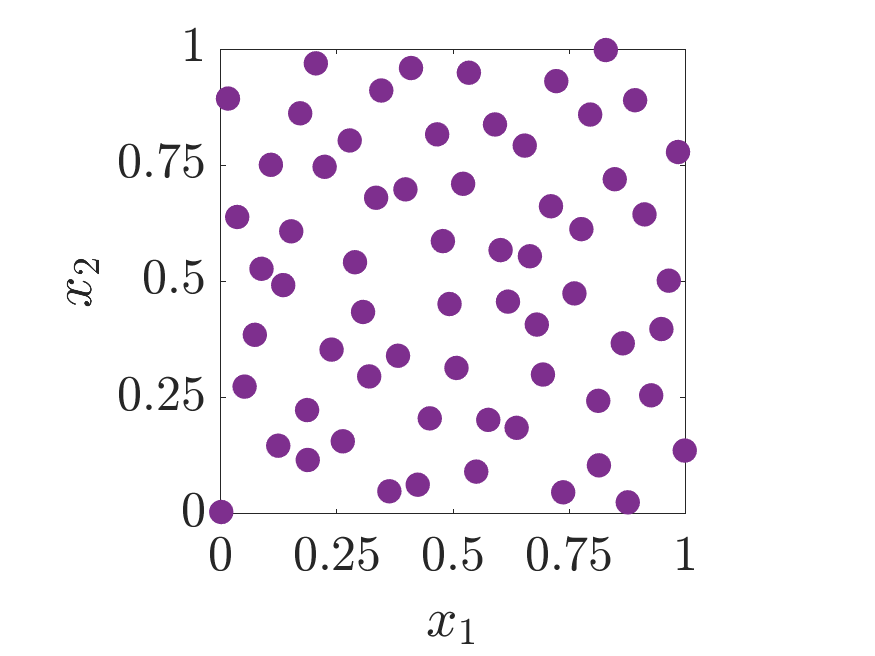
\includegraphics[width=0.8\linewidth]{figures/SSobolPoints}
	\caption{Example of a scrambled Sobol' node set  in $d=2$.  This plot can be reproduced using \code{PlotPoints.m}. }
	\label{fig:sobol-fig}
\end{figure}


\subsection{Walsh Kernels}

Walsh kernels are product kernels based on the Walsh functions. We introduce the necessary concepts in this section.

\subsubsection{Walsh functions}
Like the Fourier transform used with lattice points (\cite{RatHic19a}), the Walsh-Hadamard transform, which we will simply call Walsh transform, is used for the digital nets. The Walsh transform is defined using Walsh functions. Recall $\naturals_0 := \lbrace 0,1,2,\cdots \rbrace$.
The one-dimensional Walsh functions in base $b$ are defined as
\begin{align}
\label{eqn:walsh_func}
\textup{wal}_{b,k}(x) := e^{2\pi \sqrt{-1} (x_1 k_0 + x_2 k_1 + \cdots)/b} 
=
e^{2\pi \sqrt{-1} {\vec{k}}^T{\vec{x}}/b},
\end{align}
for $x \in [0,1)$ and $k \in \naturals_0$ and the unique base $b$ expansions 
$x = \sum_{j \ge 1} x_j b^{-i} = (0.x_1 x_2 \cdots)_b$, $\vec{x} =  (x_1,x_2,\cdots )^T$
$k = \sum_{j \ge 0} k_j b^{j} = ( \cdots k_1 k_0)_b$, $\vec{k} =  (k_0,k_1,\cdots )^T$, and ${\vec{k}}^T{\vec{x}} = x_1 k_0 + x_2 k_1 + \cdots$
where the number of digits used in \eqref{eqn:walsh_func} are limited to the length required to represent $x$ or $k$, i.e., $\max \left( {\ceil{ -\log_b{x}}, \ceil{\log_b{k}}  } \right)$.
% with $n$ at least as large as the number of digits to represent $x$ or $k$.
Multivariate Walsh functions are defined as the product of the one-dimensional Walsh functions,
\begin{align*}
\textup{wal}_{b,\vk} (\vx) := \prod_{\ell=1}^d \textup{wal}_{b,k_\ell} (x_\ell
)
\end{align*}
As shown in \eqref{eqn:walsh_func}, for the case of $b=2$, the Walsh functions only take the values in $\{1, -1\}$, i.e., $\textup{wal}_{b,\vk} : [0,1)^d \to {\{-1, 1\}} , \; k \in \naturals_0^d$. Walsh functions form an orthonormal basis of the Hilbert space $L^2[0,1)^d$,
\begin{align*}
\int_{[0,1)^d}
\textup{wal}_{b,\vl} (\vx) \textup{wal}_{b,\vk}(\vx) \dx = \delta_{\vl, \vk}, \quad \forall \vl, \vk \in \naturals_0^d
\end{align*}
Digital nets are designed to integrate certain Walsh functions without error.
Thus our Bayesian cubature algorithm integrates linear combinations of % these ideal integrands
certain Walsh functions without error. Functions that are well approximated by such linear combinations are then integrated with small errors.

% \JRNote{separate paragraph}
In this research we use Sobol' nodes which are digital nets with base $b=2$. So here afterwards base $b=2$ is assumed. % if not specified or the notation is dropped.  
In this case, the Walsh function is simply $$\textup{wal}_{2,\vk} (\vx) = (-1)^{\vec{\vk}^T \vec{\vx}}.$$

\subsubsection{Walsh kernels}
Consider the covariance kernels of the form,
\begin{align}
\label{eqn:digital_shift_in_kernel}
C_{\vtheta}(\vx, \vt) = K_{\vtheta} (\vx \ominus \vt) 
\end{align}
where $\ominus$ is bitwise subtraction.
This is called a \emph{digitally shift invariant kernel} because shifting both arguments of the covariance function by the same amount leaves the value unchanged. By a proper scaling of the function $K_{\vtheta}$, it follows that assumption \eqref{addAssump} is satisfied. The function $K_{\vtheta}$ must be of the form that ensures that $C_{\vtheta}$ is symmetric and positive definite, as assumed in \eqref{FJH:eq:CondPosDef}. We drop the ${\vtheta}$ sometimes to make the notation simpler.
The Walsh kernels are of the form,
\begin{align}
\label{eqn:walsh_kernel}
K_{\vtheta} (\vx \ominus \vt) =  
\prod_{\ell=1}^d  1 + \eta_\ell \omega_{r} (x_\ell \ominus t_\ell), \quad \veta = (\eta_1, \cdots, \eta_d), \quad \vtheta = (r, \veta)
\end{align}
where $r$ is the kernel order, $\veta$ is the kernel shape parameter, and
\begin{align*}
\omega_r(x) = \sum_{k=1}^\infty 
\frac{\textup{wal}_{2,k}(x) }{2^{2r \lfloor \log_2 k \rfloor}}.
\end{align*}
Explicit expression is available for $\omega_{r}$ in the case of order $r=1$ \cite{Nuyens2013}, % and Hilbert space setup,
\begin{align}
\label{eqn:omega1}
\omega_1(x) 
% &= \prod_{l=1}^d \sum_{k=1}^\infty 
% \frac{\textup{wal}_{b,k}(x_l) }{b^{2 \lfloor \log_b k \rfloor}} 
= 6\left( \frac 16 - 2^{\lfloor \log_2 x \rfloor -1 }\right).
\end{align}



\begin{figure}
	\centering
	\includegraphics[width=0.9\linewidth]{"figures/walsh_kernel dim_1"}
	\caption[Walsh kernel]{Walsh kernel of order $r=1$ in dimension $d=1$. This figure can be reproduced using \code{plot\_walsh\_kernel.m}. %\JRNote{remove $r=1$ in the figure}
	}
	\label{fig:walshkernel-dim1}
\end{figure}

The \figref{fig:walshkernel-dim1} shows the Walsh kernel \eqref{eqn:walsh_kernel} of order $r=1$ in the interval $[0,1)$. Unlike the shift-invariant kernels used with lattice nodes, low order Walsh kernels are discontinuous and are only piecewise constant. Smaller $\eta_\ell$ implies lesser variation in the amplitude of the kernel. Also, the Walsh kernels are digitally shift invariant but not periodic.

\subsection{Eigenvectors}

We show the eigenvectors $\mV$ in \eqref{eqn:ftk_factor} of the Gram matrix formed by the covariance kernel \eqref{eqn:walsh_kernel} and Sobol' nets are the columns of the Walsh-Hadamard matrix. First we introduce the necessary concepts.

\subsubsection{Walsh transform}
% \JRNote{add subsection for walsh transform, define and explain.}
The Walsh-Hadamard transform (WHT) is a generalized class of discrete Fourier transform (DFT) and is much simpler to compute than the DFT. The WHT matrices are comprised of only $\pm 1$ values, so the computation usually involves only ordinary additions and subtractions. Hence, the WHT is also sometimes called the integer transform. In comparison, the DFT that was used with lattice nodes,  uses complex exponential functions and the computation involves complex, non-integer multiplications. 

The WHT involves multiplications by $2^m \times 2^m$ Walsh-Hadamard matrices, which is constructed recursively, starting with $\mH^{(0)} = 1$,
\begin{align}
\nonumber
\arraycolsep=1.4pt\def\arraystretch{0.9}
\mH^{(1)} &=
\begin{pmatrix}
1 & 1 \\ 1 & -1
\end{pmatrix}, \\
\nonumber
\mH^{(2)} &= 
\begin{pmatrix}
1 & 1 & 1 & 1 \\ 
1 & -1 & 1 & -1 \\
1 & 1 & -1 & -1 \\ 
1 & -1 & -1 & 1 \\
\end{pmatrix}, \\
\nonumber
& \qquad \vdots
\\
\label{eqn:hadamard_matrix}
\mH^{(m)} &= 
\begin{pmatrix}
\mH^{(m-1)} & \mH^{(m-1)} \\ \mH^{(m-1)} & -\mH^{(m-1)}
\end{pmatrix} 
= \underbrace{\mH^{(1)} \bigotimes \cdots \bigotimes \mH^{(1)}}_{m \ \text{times}} 
= \mH^{(1)} \bigotimes \mH^{(m-1)}
\end{align}
where $\bigotimes$ is Kronecker product. Alternatively for base $b=2$, these matrices can be  directly obtained by,
\begin{align*}
\mH^{(m)} % = \bigg(\exp(\pi \sqrt{-1} \vec{\imath}_m^T\vec {\jmath}_m) \bigg)_{i,j=0}^{n-1}  
= \bigg((-1)^{(\vec{\imath}^T \vec{\jmath})} \bigg)_{i,j=0}^{2^m-1},
\end{align*}
where the notation $\vec{\imath}^T \vec{\jmath}$ indicates the bitwise dot product. 

\iffalse
An example of Walsh matrix of length $n=8$ is given in Table~\ref{tab:hadamard_matrix}. 
\begin{table} % 
	% \centering
	\arraycolsep=1pt\def\arraystretch{0.8}
	\[
	%\arraycolsep=1.4pt\def\arraystretch{0.9}
	\begin{array}{c|@{\quad}r@{\quad}r@{\quad}r@{\quad}r@{\quad}r@{\quad}r@{\quad}r@{\quad}r@{\quad}r}
	\hhline{=========}
	%\vspace{-1.5ex}
	\text{Zero crossings} & \multicolumn{8}{l}{\text{Walsh function values}} \\
	\hline
	0&	1&  1&  1&  1&  1&  1&  1&  1 \\
	4&	1& -1& -1&  1&  1& -1& -1&  1 \\
	6&	1& -1&  1& -1& -1&  1& -1&  1 \\
	2&	1&  1& -1& -1& -1& -1&  1&  1 \\
	3&	1&  1& -1& -1&  1&  1& -1& -1 \\
	7&	1& -1&  1& -1&  1& -1&  1& -1 \\
	5&	1& -1& -1&  1& -1&  1&  1& -1 \\
	1&	1&  1&  1&  1& -1& -1& -1& -1
	\end{array}
	\]
	\vspace{-5ex}
	\caption{Walsh transform matrix of for $n=8$, in Hadamard order  \label{tab:hadamard_matrix}}	   
\end{table}
\fi


\subsubsection{Eigenvectors of $\mC$ are columns of Walsh-Hadamard matrix}
\label{sec:eigenvector_hadamard}
The Gram matrix $\mCtheta$ formed by Walsh kernels and Sobol' nodes have a special structure called  block-Toeplitz, which can be used to construct the fast Bayesian transform. 
A Toeplitz matrix is a diagonal-constant matrix in which each descending diagonal from left to right is constant. A block Toeplitz matrix is a special block matrix, which contains blocks that are repeated down the diagonals of the matrix.
%, as a Toeplitz matrix has elements repeated down the diagonal. 
We prove that the eigenvectors of $\mCtheta$ are columns of a Walsh-Hadamard matrix in two theorems. 

\begin{theorem}
	\label{thrm:block-toeplitz}
	Let $\left(\vx_i\right)_{i=0}^{n-1}$ be digitally shifted Sobol' nodes and $K$ be any function,
	% positive definite kernel function such as \eqref{eqn:omega1} which matches Sobol' nodes.
	then the Gram matrix,
	\begin{align*}
	\mCtheta = \bigl(C(\vx_i, \vx_j)\bigr)_{i,j=0}^{n-1} &= \bigl(K(\vx_i \ominus \vx_j)\bigr)_{i,j=0}^{n-1},   \\ & \text{where} \quad \quad n=2^m, \quad C(\vx, \vt) = K(\vx \ominus \vt), \quad  \vx, \vt \in [0,1)^d, \qquad
	\end{align*}
	is a $2\times 2$ block-Toeplitz matrix and all the sub-blocks and their sub-sub-blocks, etc. are also $2\times 2$ block-Toeplitz. 
\end{theorem}


\iffalse
%\Subsubsection
\begin{proof}
	
	
	%\textbf{Proof of Theorem \ref{thrm:block-toeplitz}}: 
	We prove this theorem by induction. Let $\mC_{\vtheta}^{(m)}$ denote the Gram matrix of size $2^m \times 2^m$.
	The relation between sub-block matrices can be deciphered using the properties of digital nets.
	To help with the proof of block-Toeplitz structure, consider the digital net properties \eqref{eqn:digital_shift_prop},  \eqref{eqn:digital_net_symmetric_prop},
	%\begin{align*}
	%\bigl(K(\vz_i \ominus \vz_j)\bigr)_{i,j=0}^{n-1}.
	%\end{align*}
	% Now we can prove the block-Toeplitz structure using these properties and facts \JRNote{add refs to properties}.
	and notations,
	\begin{align*}
	\mK^{(m)} &:= 
	\begin{pmatrix}
	K({\vz_{i} \ominus \vz_{j}})
	\end{pmatrix}_{i,j=0}^{2^{m}-1}
	=
	\begin{pmatrix}
	K({\vz_{i \ominus j}})
	\end{pmatrix}_{i,j=0}^{2^{m}-1}, \quad m=1,2,\cdots,
	\\
	\mK^{(m,q)} &:= 
	\begin{pmatrix}
	K({\vz_{i \ominus j + q 2^m}})
	\end{pmatrix}_{i,j=0}^{2^{m}-1},
	\quad 
	q = 0,1,\cdots .
	\end{align*} 
	These two notations are related by $\mK^{(m)} = \mK^{(m,0)}$. 
	Please note that $\mC_{\vtheta}^{(m)} = \mK^{(m,0)}$.
	% Since the digitally shift invariant kernel are used in this research. %, it is sufficient to prove $\mK^{(m,q)}$ as a $2\times 2$ block-Toeplitz. 
	We will prove $\mK^{(m,q)}$ is a $2\times 2$ block-toeplitz matrix for all $m \in \naturals, q \in \naturals$.
	
	% This notation is convenient for the proof as shown below.
	
	\iffalse
	As the first step, we verify the property holds for $m=0$,
	\begin{align*}
	\mK^{(0,q)} &= \begin{pmatrix}
	K(\vz_{0 \ominus 0 + q 2^0})  
	\end{pmatrix} = 
	\begin{pmatrix}
	K(\vz_{q})
	\end{pmatrix}, \quad \text{by \eqref{eqn:digital_shift_prop}},
	\end{align*} thus by definition $\mK^{(0,q)}$ is a block-Toeplitz.
	\fi 
	
	\iftrue
	As the first step, we verify the property holds for $m=1$,
	\begin{align*}
	\mK^{(1, q)} &= \begin{pmatrix}
	K(\vz_{0 \ominus 0 + q 2^1}) & K(\vz_{1 \ominus 0 + q 2^1})  \\
	K(\vz_{0 \ominus 1 + q 2^1}) & K(\vz_{1 \ominus 1 + q 2^1})  
	\end{pmatrix} = 
	\begin{pmatrix}
	K(\vz_{2q}) & K(\vz_{1 + 2q}) \\ K(\vz_{1 + 2q}) & K(\vz_{2q})
	\end{pmatrix}, \quad \text{by \eqref{eqn:digital_shift_prop}}
	\end{align*} has diagonal elements repeated. Thus by definition, it is a $2\times 2$ block-Toeplitz.
	\fi 
	
	\iffalse
	Similarly, the property can be verified for $\mC^{(2)}$, 
	\begin{align*}
	\mC^{(2)} &= 
	\begin{pmatrix}
	K_{z_{(i \ominus j )}}
	\end{pmatrix}_{i,j=0}^{2^2-1}
	=
	\begin{pmatrix}
	K(\vz_{0 \ominus 0}) & K(\vz_{1 \ominus 0}) & K(\vz_{2 \ominus 0}) & K(\vz_{3 \ominus 0}) \\
	K(\vz_{0 \ominus 1}) & K(\vz_{1 \ominus 1}) & K(\vz_{2 \ominus 1}) & K(\vz_{3 \ominus 1}) \\
	K(\vz_{0 \ominus 2}) & K(\vz_{1 \ominus 2}) & K(\vz_{2 \ominus 2}) & K(\vz_{3 \ominus 2}) \\
	K(\vz_{0 \ominus 3}) & K(\vz_{1 \ominus 3}) & K(\vz_{2 \ominus 3}) & K(\vz_{3 \ominus 3}) 
	\end{pmatrix} \\
	& = 
	\begin{pmatrix}
	\begin{pmatrix}
	K(\vz_{0}) & K(\vz_{1}) \\
	K(\vz_{1}) & K(\vz_{0})
	\end{pmatrix} &
	\begin{pmatrix}
	K(\vz_{2}) & K(\vz_{3}) \\
	K(\vz_{3}) & K(\vz_{2}) 
	\end{pmatrix} \\
	\begin{pmatrix}
	K(\vz_{2}) & K(\vz_{3}) \\
	K(\vz_{3}) & K(\vz_{2}) 
	\end{pmatrix} &
	\begin{pmatrix}
	K(\vz_{0}) & K(\vz_{1}) \\
	K(\vz_{1}) & K(\vz_{0})
	\end{pmatrix} 
	\end{pmatrix}, \quad \text{by \eqref{eqn:digital_shift_prop}, \eqref{eqn:digital_net_symmetric_prop}}
	\\
	& =
	\begin{pmatrix}
	\mC^{(1)} & \mC^{(1,1)} \\
	\mC^{(1,1)} & \mC^{(1)}
	\end{pmatrix},
	\end{align*}
	is a block-Toeplitz as it is obvious from the block structure depicted. 
	\fi
	% Here we used the notation $\mC^{(1,1)}$ to indicate the additional operation involved in the matrix.
	% Where the matrix $\mC^{(1,1)}$ is obtained using the following shift operation.
	
	Now assume that $\mK^{(m,q)}$ is block-Toeplitz.
	% Please note if $\mK^{(m,0)}$ is block-Toeplitz then $\mK^{(m,q)}$ is also a block-Toeplitz for all $q \in \naturals_0$. 
	% This is due to the fact that $i \oplus 2^m \ominus j = i \ominus j \ominus 2^m = i \ominus j \oplus 2^m $ for $i,j=0,\cdots,2^{m-1}$ since $i \ominus j < 2^{m-1}$.
	% Assuming $\mK^{(m, q)}$ is a block-Toeplitz, 
	We need to prove $\mK^{(m+1, q)}$ is also a $2\times 2$ block-Toeplitz. Let $n=2^m$,
	\begin{align*}
	\mK^{(m+1)} &= 
	\begin{pmatrix}
	K(\vz_{0    \ominus 0}) & \hdots & K(\vz_{0    \ominus n-1}) & K(\vz_{0    \ominus n}) & \hdots & K(\vz_{0    \ominus 2n-1}) \\
	\vdots             & \vdots &             \vdots          &           \vdots      & \vdots &             \vdots         \\
	K(\vz_{n-1  \ominus 0}) & \hdots & K(\vz_{n-1  \ominus n-1}) & K(\vz_{n-1  \ominus n}) & \hdots & K(\vz_{n-1  \ominus 2n-1}) \\
	K(\vz_{n    \ominus 0}) & \hdots & K(\vz_{n    \ominus n-1}) & K(\vz_{n    \ominus n}) & \hdots & K(\vz_{n    \ominus 2n-1}) \\
	\vdots      & \vdots &             \vdots        &             \vdots      & \vdots &             \vdots         \\
	K(\vz_{2n-1 \ominus 0}) & \hdots & K(\vz_{2n-1 \ominus n-1}) & K(\vz_{2n-1 \ominus n}) & \hdots & K(\vz_{2n-1 \ominus 2n-1}) 
	\end{pmatrix} 
	\\
	& = 
	\begin{pmatrix}
	\begin{pmatrix}
	K(\vz_{  0   }) & \hdots & K(\vz_{ n-1}) \\
	\vdots          & \vdots &    \vdots     \\
	K(\vz_{ n-1  }) & \hdots & K(\vz_{ 0 })
	\end{pmatrix}
	& 
	\begin{pmatrix}
	K(\vz_{ n})     & \hdots & K(\vz_{ 2n-1}) \\
	\vdots          & \vdots &     \vdots     \\
	K(\vz_{ 2n-1 }) & \hdots & K(\vz_{ n })   
	\end{pmatrix}
	\\
	\begin{pmatrix}
	K(\vz_{ n})     & \hdots & K(\vz_{ 2n-1}) \\
	\vdots          & \vdots &     \vdots     \\
	K(\vz_{ 2n-1 }) & \hdots & K(\vz_{ n })   
	\end{pmatrix}
	&
	\begin{pmatrix}
	K(\vz_{  0   }) & \hdots & K(\vz_{ n-1}) \\
	\vdots          & \vdots &    \vdots     \\
	K(\vz_{ n-1  }) & \hdots & K(\vz_{ 0 })
	\end{pmatrix}
	\end{pmatrix} 
	\\
	& =
	\begin{pmatrix}
	\mK^{(m)} & \mK^{(m,1)} \\ \mK^{(m,1)} & \mK^{(m)}
	\end{pmatrix}
	\end{align*}
	is a $2\times 2$ block-Toeplitz, where we used the properties  \eqref{eqn:digital_shift_prop}, \eqref{eqn:digital_net_symmetric_prop} and facts $2n-1 \ominus n = n-1$, $2n-1 \ominus n-1 = n$, and $n \ominus n-1 = 2n-1$. 
	Thus $\mK^{(m+1)}$ is a $2\times2$ block-Toeplitz. 
	Similarly 
	\begin{align*}
	\mK^{(m+1,q)} 
	& =
	\begin{pmatrix}
	\mK^{(m,q)} & \mK^{(m,q+1)} \\ \mK^{(m,q+1)} & \mK^{(m,q)}
	\end{pmatrix}
	\end{align*}
	is a $2\times2$ block-Toeplitz. 
	%\end{itemize}
	Thus $\mC_{\vtheta}^{(m)}$ of size $2^m\times 2^m$, for $m \in \naturals$, is a $2\times2$ block-Toeplitz and every block and it's sub-blocks of size $2^p, \; p \in \naturals, \; p \le m$ are also $2\times2$ block-Toeplitz.
\end{proof}
\fi

%%%%%%%%%%%%%%%%%%%%%%%%%%%%%%%%%%%%%%%%%%%%%%%%%%%%%%%%%%%%%%%%%%%%%%%%%%%%%%%

\iffalse
Some additional properties
$\bigl( K(z_{i \ominus j})\bigr)_{i=2^{l+1}q, \; j=2^{l+1}s}^{2^{l+1}{(q+1)}, \; 2^{l+1}{(s+1)}} $
\fi



\iffalse
Now we prove every arbitrary sub-block is also block-Toeplitz: 
\begin{itemize}
	\item For $l=1$
	\begin{align*}
	\bigl( K(z_{i \ominus j})\bigr)_{i=2q, \; j=2s}^{2q+1, 2s+1}, \quad q,s=0,1,\cdots,
	\end{align*}
	is a block-Toeplitz since
	\begin{align*}
	\begin{pmatrix}
	K(z_{2q \ominus 2s}) & K(z_{2q \ominus (2s +1)}) \\
	K(z_{(2q+1) \ominus 2s}) & K(z_{(2q+1) \ominus (2s +1)}) 
	\end{pmatrix}
	=
	\begin{pmatrix}
	K(z_{2q \ominus 2s}) & K(z_{1 + (2q \ominus 2s)}) \\
	K(z_{1 + (2q \ominus 2s)}) & K(z_{ 2q \ominus 2s}) 
	\end{pmatrix}
	\end{align*}
	where we used the facts $(2q+1) \ominus (2s+1) = 2q \ominus 2s$ and $(2q+1) \ominus 2s = 1 + 2q \ominus 2s$.
	
	\item \ldots
	
	\item Assuming for $2^{l}$ is a block-Toeplitz then need to prove for $2^{l+1}$ 
	\begin{align*}
	\bigl( K(z_{i \ominus j})\bigr)_{i=2^{l+1}q, \; j=2^{l+1}s}^{2^{l+1}(q+1)-1, \; 2^{l+1}(s+1)-1}, \quad q,s=0,1,\dots,
	\end{align*}
	is a block-Toeplitz.
	
	\begin{align*}
	\mC &=
	\begin{pmatrix}
	\bigl( K(z_{i \ominus j})\bigr)_{i=\ia, \; j=\ja }^{\ib, \; \jb} & \bigl( K(z_{i \ominus j})\bigr)_{i=\ia, \; j=\jc }^{\ib, \; \jd} \\
	\bigl( K(z_{i \ominus j})\bigr)_{i=\ic, \; j=\ja }^{\id, \; \jb} & \bigl( K(z_{i \ominus j})\bigr)_{i=\ic, \; j=\jc }^{\id, \; \jd}
	\end{pmatrix} \\
	& =
	\begin{pmatrix}
	\bigl( K(z_{i \ominus j})\bigr)_{i=\ia, \; j=\ja }^{\ib, \; \jb} & \bigl( K(z_{i \ominus j})\bigr)_{i=\ia, \; j=\jc }^{\ib, \; \jd} \\
	\bigl( K(z_{i \ominus j})\bigr)_{i=\ia, \; j=\jc }^{\ib, \; \jd} & \bigl( K(z_{i \ominus j})\bigr)_{i=\ia, \; j=\ja }^{\ib, \; \jb}
	\end{pmatrix}
	\end{align*}
	is a block-Toeplitz. Where we used the facts
	\begin{align*}
	% \ic \ominus \jc 
	& 2^{l}(2q+1) \ominus 2^{l}(2s+1) = 2^{l}(2q) \ominus 2^{l}(2s) = 2^{l+1}(q) \ominus 2^{l+1}(s) \\
	% \jd \ominus \ic
	&2^{l+1}(s+1)-1 \, \ominus 2^{l}(2q + 1) % = 2^{l}(2s+1 + 1)-1 \ominus 2^{l}(2q + 1) 
	= 2^{l}(2s+1)-1 \ominus 2^{l+1}q.
	\end{align*}
	
	Thus $\mCtheta^{(m)}$ is a block-Toeplitz and every block its and sub-blocks are also block-Toeplitz.
	
	
\end{itemize}
\fi


\begin{theorem}
	\label{thrm:hadamard_eigenvector}
	The Walsh-Hadamard matrix $\mH^{(m)}$ factorizes $\mC_{\vtheta}^{(m)}$, so that the columns of Walsh-Hadamard matrix are the eigenvectors of $\mC_{\vtheta}^{(m)}$, i.e.,
	\begin{align*}
	\mH^{(m)} \mC_{\vtheta}^{(m)}  = \mLambda^{(m)} \mH^{(m)}, \quad m \in \naturals. 
	\end{align*}
\end{theorem}

A detailed proof for Theorem \ref{thrm:block-toeplitz} and \ref{thrm:hadamard_eigenvector} can be found in \cite{JagThesis19a}.

\iffalse
\begin{proof}
	
	Again, we use the proof-by-induction technique to show that the Walsh-Hadamard matrix factorizes $\mK^{(m,q)}$.
	\iffalse
	We can easily see the Hadamard matrix $\mH^{(0)}$ diagonalizes $\mC^{(0)}$,
	\begin{align*}
	\mH^{(0)} \mC^{(0)} &= 
	\begin{pmatrix}
	1 
	\end{pmatrix}
	\begin{pmatrix}
	K(\vz_{0}) 
	\end{pmatrix}
	\\
	% & = \begin{pmatrix} K(\vz_{0})+K(\vz_{1}) & K(\vz_{0})+K(\vz_{1}) \\ K(\vz_{0})-K(\vz_{1}) & K(\vz_{1})-K(\vz_{0}) \end{pmatrix} \\ 
	& = 
	\begin{pmatrix}
	K(\vz_{0})
	\end{pmatrix}
	\begin{pmatrix}
	1 
	\end{pmatrix}
	\\ 
	% & = \begin{pmatrix} K(\vz_{0})+K(\vz_{1}) & 0 \\ 0 & K(\vz_{0})-K(\vz_{1}) \end{pmatrix} \mH^{(1)} \\
	&= \mLambda^{(0)} \mH^{(0)},
	\end{align*}
	where $\mLambda^{(0)}$ is a diagonal matrix, thus $\mH^{(0)}$ diagonalizes $\mC^{(0)}$.
	\fi
	We can easily see the Hadamard matrix $\mH^{(1)}$ diagonalizes $\mK^{(1,q)}$,
	\begin{align*}
	\mH^{(1)} \mK^{(1,q)} &= 
	\begin{pmatrix}
	1 &  1 \\ 1 & -1
	\end{pmatrix}
	\begin{pmatrix}
	K(\vz_{0 + q2^1}) & K(\vz_{1 + q2^1}) \\ K(\vz_{1 + q2^1}) & K(\vz_{0 + q2^1})
	\end{pmatrix}, \quad \text{by Theorem \ref{thrm:block-toeplitz}} 
	\\
	& = \begin{pmatrix} K(\vz_{2q})+K(\vz_{2q+1}) & K(\vz_{2q})+K(\vz_{2q+1}) \\ K(\vz_{2q})-K(\vz_{2q+1}) & K(\vz_{2q+1})-K(\vz_{2q}) \end{pmatrix} \\ 
	& = \begin{pmatrix} K(\vz_{2q})+K(\vz_{2q+1}) & 0 \\ 0 & K(\vz_{2q})-K(\vz_{2q+1}) \end{pmatrix} 
	\begin{pmatrix}
	1 &  1 \\ 1 & -1
	\end{pmatrix} \\
	&= \mLambda^{(1,q)} \mH^{(1)},
	\end{align*}
	where $\mLambda^{(1,q)}$ is a diagonal matrix, thus $\mH^{(1)}$ factorizes $\mK^{(1,q)}$.
	
	Now assume $\mH^{(m)}$ factorizes $\mK^{(m,q)}$, so $\mH^{(m)} \mK^{(m,q)} = \mLambda^{(m,q)} \mH^{(m)}$ where $\mLambda^{(m,q)}$ is diagonal. We need to prove $\mH^{(m+1)}$ factorizes $\mK^{(m+1,q)}$,
	\begin{align*}
	\mH^{(m+1)} \mK^{(m+1,q)} &= 
	\begin{pmatrix}
	\mH^{(m)} & \mH^{(m)} \\ \mH^{(m)} & -\mH^{(m)}
	\end{pmatrix}
	\begin{pmatrix}
	\mK^{(m,q)} & \mK^{(m,q+1)} \\ \mK^{(m,q+1)} & \mK^{(m,q)}
	\end{pmatrix}, \quad \text{by Theorem \ref{thrm:block-toeplitz}}
	\\
	& = \begin{pmatrix}
	\mH^{(m)} (\mK^{(m,q)}   + \mK^{(m,q+1)}) & 
	\mH^{(m)} (\mK^{(m,q)}   + \mK^{(m,q+1)}) \\ 
	\mH^{(m)} (\mK^{(m,q)}   - \mK^{(m,q+1)}) & 
	\mH^{(m)} (\mK^{(m,q+1)} - \mK^{(m,q)}) 
	\end{pmatrix} \\ 
	& = \begin{pmatrix}
	(\mLambda^{(m,q)}  + \mLambda^{(m,q+1)})  \mH^{(m)} & 
	(\mLambda^{(m,q)}   + \mLambda^{(m,q+1)}) \mH^{(m)} \\ 
	(\mLambda^{(m,q)}   - \mLambda^{(m,q+1)}) \mH^{(m)} & 
	(\mLambda^{(m,q+1)} - \mLambda^{(m,q)})   \mH^{(m)}
	\end{pmatrix} \\ 
	& = 
	\begin{pmatrix}
	\mLambda^{(m,q)} + \mLambda^{(m,q+1)} & 0 \\ 0 & \mLambda^{(m,q)} - \mLambda^{(m,q+1)}
	\end{pmatrix}
	\begin{pmatrix}
	\mH^{(m)} & \mH^{(m)} \\ \mH^{(m)} & -\mH^{(m)}
	\end{pmatrix}
	\\ 
	% & = \begin{pmatrix} \mC^{(m)} + \mC^{(m,m)} & 0 \\ 0 & \mC^{(m)} - \mC^{(m,m)} \end{pmatrix} \mH^{(m+1)} \\
	& = \mLambda^{(m+1,q)} \mH^{(m+1)} .
	\end{align*}
	Thus, $\mH^{(m+1)}$ factorizes $\mK^{(m+1,q)}$ to a diagonal matrix $\mLambda^{(m+1,q)}$. This implies $\mH^{(p)}$ factorizes $\mC_\vtheta^{(p)}$ for $p \in \naturals$. Please recall $\mC_\vtheta^{(p)} = \mK^{(p,0)}$.  Here we used the fact that both $\mH$ and $\mK$ are symmetric positive definite. 
\end{proof}
\fi

\iffalse
Next, we show the eigenvectors of a block-Toeplitz matrix can be obtained by Kronecker product of its sub-block matrices. If $\mA, \mB$ share same eigenvalues $\mA \mV = \mLambda \mV, \mB \mV = \mV \mSigma$ then
\begin{align*}
\begin{pmatrix}
\mA & \mB \\ \mB & \mA
\end{pmatrix}
\begin{pmatrix}
\mV & \mV \\ \mV & -\mV
\end{pmatrix}
= 
\begin{pmatrix}
\mV & \mV \\ \mV & -\mV
\end{pmatrix}
\begin{pmatrix}
\mLambda + \mSigma & 0 \\ 0 & \mLambda - \mSigma 
\end{pmatrix}
\end{align*}
\fi


\subsection{Fast Bayesian transform}
We can easily show that the Walsh-Hadamard matrices satisfy the assumptions of fast Bayesian transform \eqref{fastcompAssump}. As shown in Section~\ref{sec:eigenvector_hadamard} the columns of $\mH^{({m})}$ are the eigenvectors. Since the Gram matrix $\mC$ is symmetric, the columns/rows of Walsh-Hadamard matrices are mutually orthogonal. Thus the Gram matrix can be written as 
\begin{align}
\label{eqn:hadamard_fwht}
\mC^{(m)} = \frac{1}{n} \mH^{(m)} \mLambda^{(m)} \mH^{(m)}, \quad \text{where} \quad \mH^{({m})} = \underbrace{ \mH^{(1)} \bigotimes \cdots \bigotimes \mH^{(1)} }_{m \; \text{times}}.
\end{align}
% \JRNote{prove eigenvalues for Sobol case}
Assumption \eqref{fastcompAssumpB} follows automatically by the fact that Walsh-Hadamard matrices can be constructed analytically. Assumption \eqref{fastcompAssumpA} can also be verified as the first row/column are one vectors. Finally, assumption \eqref{fastcompAssumpC} is satisfied due to the fact that fast Walsh transform can be computed in $\Order({n \log n})$ operations using fast Walsh-Hadamard transform.
Thus the Walsh-Hadamard transform is a fast Bayesian transform, $\mV := \mH$, as per \eqref{fastcompAssump}.

We have implemented a fast adaptive Bayesian cubature algorithm using the kernel \eqref{eqn:walsh_kernel} with $r=1$ and Sobol' points \cite{BraFox88} in MATLAB as part of the Guaranteed Adaptive Integration Library (GAIL) \cite{ChoEtal17b} as \allowbreak \code{cubBayesNet\_g}. The Sobol' points used in this algorithm are generated using MATLAB's builtin function \code{sobolset} and scrambled using MATLAB function \code{scramble} \cite{HonHic00a}. The fast Walsh-Hadamard transform \eqref{eqn:hadamard_fwht} is computed using MATLAB's builtin function \code{fwht} with \emph{hadamard} ordering. 

\subsection{Iterative Computation of Walsh Transform}
In every iteration of our algorithm, we double the number of function values. Using the technique described here, we have to only compute the Walsh transform for the newly added function values.
Similar to the lattice points, Sobol' points are extensible by definition. This property is used in our algorithm to improve the integration accuracy till the required error tolerance is met. Sobol' nodes can be combined with Hadamard matrices as demonstrated here for iterative computation. 
% Using the same notations as in \secref{sec:iter_fft}, l
Let $\widetilde{\vy} = \mH^{(m+1)} {\vy}$ for some arbitrary $\vy \in \reals^{2n}$, $n = 2^m$. Define, 
\begin{gather*}
\vy = \begin{pmatrix} y_1 \\ \vdots \\ y_{2n} \end{pmatrix}, \quad 
\vy^{(1)} = \begin{pmatrix} y_1 \\ \vdots \\ y_{n} \end{pmatrix}, \quad 
\vy^{(2)}  = \begin{pmatrix} y_{n+1} \\ \vdots \\ y_{2n} \end{pmatrix}, \\ 
\widetilde{\vy}^{(1)} = \mH^{(m)} \vy^{(1)} = 
\begin{pmatrix} \widetilde{y}^{(1)}_1 \\ \widetilde{y}^{(1)}_2 \\ \vdots \\ \widetilde{y}^{(1)}_{n} \end{pmatrix}, \quad 
\widetilde{\vy}^{(2)}  =  \mH^{(m)} \vy^{(2)} =
\begin{pmatrix} \widetilde{y}^{(2)}_{1} \\  \widetilde{y}^{(2)}_{2} \\ \vdots \\ \widetilde{y}^{(2)}_{n} \end{pmatrix}. 
\end{gather*}
Then,
\begin{align*}
\widetilde{\vy} &= \mH^{({m+1})} {\vy} \\
& = \begin{pmatrix}
\mH^{(m)} & \mH^{(m)} \\ \mH^{(m)} & - \mH^{(m)}
\end{pmatrix} 
\begin{pmatrix}
\vy^{(1)} \\ \vy^{(2)}
\end{pmatrix}, \qquad \text{by \eqref{eqn:hadamard_matrix}} \\
&= 
\begin{pmatrix}
\mH^{(m)} \vy^{(1)} + \mH^{(m)} \vy^{(2)} \\ 
\mH^{(m)} \vy^{(1)} - \mH^{(m)} \vy^{(2)}
\end{pmatrix}\\
&= 
\begin{pmatrix}
\widetilde{\vy}^{(1)} + \widetilde {\vy}^{(2)} \\ 
\widetilde {\vy}^{(1)} - \widetilde {\vy}^{(2)}
\end{pmatrix} =: \widetilde{\vy} \quad.
\end{align*}
As before with the lattice nodes, the computational cost to compute $\mV^{(m+1)H} \vy$ is 
twice the cost of computing $\mV^{(m)H} \vy^{(1)}$ plus $2n$ additions, where $n=2^m$. An inductive argument shows that for any $m \in \naturals$, $\mV^{(m)H}\vy$ requires only $\Order(n \log n)$ operations. Usually the multiplications in $\mV^{(m)H} \vy^{(1)}$ are multiplications by $-1$ which are simply accomplished using sign change or negation, requiring no multiplications at all.


\subsection{Higher Order Nets}

Higher order digital nets are an extension of $(t,m,d)$-nets, introduced in \cite{Dic08a}. They can be used to numerically integrate smoother functions which are not necessarily periodic, but have square integrable mixed partial derivatives of order $\alpha$, at a rate of $\Order(n^{-\alpha})$ multiplied by a power of a $\log n$ factor using rules corresponding to the modified $(t,m, d)$-nets.
We want to emphasize that quasi-Monte Carlo rules based on these point sets can achieve convergence rates faster than $\Order(n^{-1})$. 
Higher order digital nets are constructed using matrix-vector multiplications over finite
fields. 

One could develop matching digitally shift invariant kernels to formulate the fast Bayesian cubature. Bayesian cubatures using higher order digital nets are a topic for future research.





















%%%%%%%%%%%%%%%%%%%%%%%%%%%%%%%%%%%%%%%%%%%%%%%%%%%%%%%%%%%%%%%%%%%%%%%%%%%%%%%%%%%%%%%%%%%%%%%%%%%%%%%%%%%%%%%%%%%%%%%%%%%%%%%%%%%%%%%%%%%%%%%%%%%%%%%%%%%%%%%%%%%%%%%%%%%%%%%%%%%%



\section{Numerical Experiments}

\label{sec:NumExp}

\JRNote{use uniformly randomly chosen $\varepsilon$ instead 4 fixed}

Fast Bayesian cubature algorithms developed in this research are demonstrated using three commonly used integration examples.
These integrals are evaluated using our algorithm \code{cubBayesNet\_g} and compared with \code{cubBayesLattice\_g} which was developed in \cite{RatHic19a}. The \code{cubBayesLattice\_g} is a fast automatic Bayesian cubature algorithm which uses rank-1 lattice nodes. The first example shows evaluating a multivariate Gaussian probability given the interval. The second example shows integrating the Keister's function, and the final example shows computing an Asian arithmetic option pricing.  


\subsection{Testing Methodology}
\label{sec:numerical_experiments_cubBayesLattice}

% Three integrals were evaluated using our GAIL algorithms:  a multivariate Gaussian probability, the Keister's example, and an option pricing example. 
Four hundred different error tolerances, $\varepsilon$, were randomly chosen from a fixed interval  for each example. 
The intervals for error tolerance were chosen depending on the difficulty of the problem.
The nodes used in \code{cubBayesNet\_g} were the randomly scrambled and shifted Sobol' points supplied by MATLAB's Sobol' sequence generator. 

For each integral example, and each stopping criteria---empirical Bayes, full Bayes, and generalized cross-validation---our algorithm is run with each randomly chosen error tolerance as mentioned above.  For each test, the execution time is plotted against $\abs{\mu - \hmu}/\varepsilon$.  We expect $\abs{\mu - \hmu}/\varepsilon$ to be no greater than one, but hope that it is not too much smaller than one, which would indicate a stopping criterion that is too conservative.
%Unlike the examples in previous \secref{sec:numerical_experiments_cubBayesLattice}, periodization variable transform is not required.


Periodization variable transforms are not used in the examples with \\ \allowbreak \code{cubBayesNet\_g}. Since the \allowbreak \code{cubBayesNet\_g} does not need periodized integrands, so the integrands are used directly.

% \Section{Test Results and Observations for \code{cubBayesNet\_g}}
% \label{sec:numerical_experiments_cubBayesNet}

%Similar to the previous examples, we used four different error tolerances, $\varepsilon$,  set for each example, with the tolerances chosen depending on the difficulty of the problem.  
%For each integral,  each tolerance, and each of our stopping criteria---empirical Bayes, full Bayes, and generalized cross-validation---our algorithm is run  $100$ times.  For each test, the execution time is plotted against $\abs{\mu - \hmu}/\varepsilon$.  
% We expect $\abs{\mu - \hmu}/\varepsilon$ to be no greater than one, but hope that it is not too much smaller than one, which would indicate a stopping criterion that is too conservative. 

\subsection{Multivariate Gaussian Probability}

This example was introduced in \cite{RatHic19a}, where we used with the Mat\'ern covariance kernel and shift-invariant kernel. 
Here we use $ f_{\textup{Genz}}$ \eqref{eqn:fGenzdef} without any periodization as it is not required, and chose $d=3$ and $r=1$, where 
\begin{equation}
	\label{eqn:fGenzdef}
	f_{\textup{Genz}}(\vx) = \prod_{j=1}^d [\beta_j(\vx) - \alpha_j(\vx)].
\end{equation}
The simulation results for this example integrand are summarized in Figures \ref{fig:Sobol-mvn-guaranteed-MLE}, \ref{fig:Sobol-mvn-guaranteed-FB}, and \ref{fig:Sobol-mvn-guaranteed-GCV}.  In all cases, {\code{cubBayesNet\_g} returns an approximation within the prescribed error tolerance. We used the same setting as before with generic slow Bayesian cubature in \cite{RatHic19a} for comparision. For error threshold $\varepsilon=10^{-5}$ with empirical stopping criterion, our fast algorithm takes about 2 seconds as shown in \figref{fig:Sobol-mvn-guaranteed-MLE} whereas the basic algorithm takes 30 seconds as shown in \cite{RatHic19a}. 
{\code{cubBayesNet\_g} uses fast Walsh transform which is slower in MATLAB due to the way it was implemented. This is reason it takes more longer the {\code{cubBayesLattice\_g}. 
But comparing the number of samples, $n$, used for integration provides more insight which directly relates to alogrithm's computational cost. The {\code{cubBayesLattice\_g} used $n=16384$ samples whereas {\code{cubBayesNet\_g} used $n=32768$ samples even with $r=1$ order kernel.

Amongst the three stopping criteria, GCV achieved the results faster than others but it is less conservative. 
One can also observe from the figures that the credible intervals are narrower than in \figref{fig:Sobol-mvn-guaranteed-MLE}.
This shows that {\code{cubBayesNet\_g} with $r=1$ kernel more accurately approximates the integrand.

\begin{figure}
\centering
%d=3 problem transformed into d=2
\includegraphics[width=0.95\linewidth]{"figures/Sobol/Sobol_MVN_guaranteed_time_MLE__d2_r1_2019-Sep-1"}
\caption[Sobol: MVN guaranteed: MLE]{Multivariate normal probability example with empirical Bayes stopping criterion.}
\label{fig:Sobol-mvn-guaranteed-MLE}
\end{figure}
\begin{figure}
\centering
%d=3 problem transformed into d=2
\includegraphics[width=0.95\linewidth]{"figures/Sobol/Sobol_MVN_guaranteed_time_full__d2_r1_2019-Sep-1"}
\caption[Sobol: MVN guaranteed: Full Bayes]{Multivariate normal probability example with the full-Bayes stopping criterion.}
\label{fig:Sobol-mvn-guaranteed-FB}
\end{figure}
\begin{figure}
\centering
%d=3 problem transformed into d=2
\includegraphics[width=0.95\linewidth]{"figures/Sobol/Sobol_MVN_guaranteed_time_GCV__d2_r1_2019-Sep-1"}
\caption[Sobol: MVN guaranteed: GCV]{Multivariate normal probability example with the GCV stopping criterion.}
\label{fig:Sobol-mvn-guaranteed-GCV}
\end{figure}






\subsection{Keister's Example}

This multidimensional integral function comes from \cite{Kei96} and is inspired by a physics application:
\begin{align}
\label{eqn:keister_integral}
\mu & =  \int_{\reals^d} \cos(\norm{ \vt}) \exp(-\norm{ \vt }^2) \, \dvt \\
\nonumber
%&  = 
%\int_{\reals^d} \cos(a\norm{ \vt}) \exp(-a^2\norm{ \vt }^2)  a^d \, \dvt \\
& = \int_{[0,1]^d} f_{\textup{Keister}}(\vx) \, \dvx,\\
\intertext{where }
\nonumber
f_\textup{Keister}(\vx) &= \pi^{d/2} \cos\left(\norm{ \Phi^{-1}(\vx)/2}\right)  ,
\end{align}
and $\Phi$ is the standard normal distribution.
%\begin{figure}
%	\captionsetup[subfigure]{labelformat=empty}
%	\begin{subfigure}[h]{0.48\linewidth}
%		\includegraphics[width=1.1\linewidth]{Keister_wholeR_1D}
%	\end{subfigure}
%	\begin{subfigure}[h]{0.48\linewidth}
%		\includegraphics[width=1.1\linewidth]{Keister_cube_1D}
%	\end{subfigure}
%	\caption{Keister function in d=2 and its transformed version in $[0,1]^2$ with various values of $a$.}
%	\label{fig:keister}
%\end{figure}
The true value of $\mu$ can be calculated iteratively in terms of a quadrature as follows:  
\begin{equation*}
\mu = \frac{2 \pi^{d/2} I_c(d)}{\Gamma(d/2)}, \quad d=1,2, \ldots
\end{equation*}
where $\Gamma$ denotes the gamma function, and
\begin{align*}
I_c(1) &= \frac{\sqrt{\pi}}{2 \exp(1/4)}, 
\\
I_s(1) &= \int_{x=0}^\infty \exp(-\vx^T\vx)\sin(\vx) \, \dvx 
\\
& =  0.4244363835020225,
\\
I_c(2) &= \frac{1-I_s(1)}{2}, \qquad
I_s(2) = \frac{I_c(1)}{2}
\\
I_c(j) &= \frac{(j-2)I_c(j-2)-I_s(j-1)}{2},
\qquad j =3,4,\ldots
\\
I_s(j) &= \frac{(j-2)I_s(j-2)-I_c(j-1)}{2},
\qquad j =3,4,\ldots.
% ref: https://www.mathworks.com/help/matlab/ref/gamma.html
\end{align*}


Figures \ref{fig:Sobol-keister-guaranteed-MLE}, \ref{fig:Sobol-keister-guaranteed-FB} and \ref{fig:Sobol-keister-guaranteed-GCV} summarize the numerical tests for this case. We used  dimension $d=4$, and $r=1$.  No periodization transform was used as the integrand need not be periodic. 
In this example, we use $r=1$ order kernel whereas \code{cubBayesLattice\_g} in \cite{RatHic19a}, $r=2$ kernel was used. This necessitates \code{cubBayesNet\_g} to use more samples for integration.
As observed from the figures, the GCV stopping criterion achieved the results faster than the others but it is less conservative which is also the case with the multivariate Gaussian example.

\begin{figure}
\centering
\includegraphics[width=0.95\linewidth]{"figures/Sobol/Sobol_Keister_guaranteed_time_MLE__d4_r1_2019-Sep-1"}
\caption[Sobol: Keister guaranteed: MLE]{Keister example using the empirical Bayes stopping criterion.}
\label{fig:Sobol-keister-guaranteed-MLE}
\end{figure}
\begin{figure}
\centering
\includegraphics[width=0.95\linewidth]{"figures/Sobol/Sobol_Keister_guaranteed_time_full__d4_r1_2019-Sep-1"}
\caption[Sobol: Keister guaranteed: Full Bayes]{Keister example using the full-Bayes stopping criterion.}
\label{fig:Sobol-keister-guaranteed-FB}
\end{figure}
\begin{figure}
\centering
\includegraphics[width=0.95\linewidth]{"figures/Sobol/Sobol_Keister_guaranteed_time_GCV__d4_r1_2019-Sep-1"}
\caption[Sobol: Keister guaranteed: GCV]{Keister example using the GCV stopping criterion.}
\label{fig:Sobol-keister-guaranteed-GCV}
\end{figure}







\subsection{Option Pricing}

The price of financial derivatives can often be modeled by high dimensional integrals. If the underlying asset is described in terms of a discretized geometric Brownian motion, then the fair price of the option is:
\begin{equation*}
\mu = \int_{\reals^d} \text{payoff}(\vz) \frac{\exp(\frac 12 \vz^T\mSigma^{-1}\vz)}{\sqrt{(2\pi)^d \det(\mSigma)}} \, \dvz = \int_{[0,1]^d} f(\vx) \, \dvx,
\end{equation*} 
where {payoff($\cdot$)} defines the discounted payoff of the option,
\begin{align*}
\mSigma &= (T/d) \bigl(\min(j,k) \bigr)_{j,k=1}^d = \mL \mL^T,\\
f(\vx) &= \text{payoff} \left(\mL 
\begin{pmatrix}
\Phi^{-1}(x_1) \\ \vdots \\ \Phi^{-1}(x_d)
\end{pmatrix} \right).
\end{align*}
The Asian arithmetic mean call option has a payoff of the form
\begin{align*}
\text{payoff}(\vz) &= \max\left( \frac 1d  \sum_{j=1}^d S_j(\vz) - K, 0 \right) \me^{-r T}, \\
S_j(\vz) &= S_0 \exp\bigl((r-\sigma^2/2)jT/d + \sigma \sqrt{T/d} z_j \bigr).
\end{align*}
Here, $T$ denotes the time to maturity of the option, $d$ the number of time steps, $S_0$ the initial price of the stock, $r$ the interest rate, $\sigma$ the volatility, and $K$ the strike price.  

%\Subsection{Option Pricing}
The Figures \ref{fig:Sobol-optprice-guaranteed-MLE}, \ref{fig:Sobol-optprice-guaranteed-FB} and 
\ref{fig:Sobol-optprice-guaranteed-GCV} summarize the numerical results for the option pricing example using the values for,
$
T = 1/4, \ \ d = 13, \ \ S_0 = 100, \ \ r =  0.05, \ \ \sigma = 0.5, \ \ K = 100
$, same as used in the experiments of \code{cubBayesLattice\_g} \cite{RatHic19a}.
As mentioned before, this integrand has a kink caused by the $\max$ function, so, \code{cubBayesNet\_g} could be more efficient than \code{cubBayesLattice\_g}, as no periodization transform is required. This can be observed from the number of samples used for intgration to meet the same error threshold. For the error tolerance, $\varepsilon=10^{-3}$,  \code{cubBayesLattice\_g} used $n=2^{20}$ samples, whereas \code{cubBayesNet\_g} used $n=2^{17}$ samples.


\begin{figure}
\centering
\includegraphics[width=0.95\linewidth]{"figures/Sobol/Sobol_optPrice_guaranteed_time_MLE__d12_r1_2019-Sep-1"}
\caption[Sobol: Option pricing guaranteed: MLE]{Option pricing using the empirical Bayes stopping criterion. The hollow stars indicate the algorithm has not met the error threshold $\epsilon$ even with using maximum $n$.}
\label{fig:Sobol-optprice-guaranteed-MLE}
\end{figure}
\begin{figure}
\centering
\includegraphics[width=0.95\linewidth]{"figures/Sobol/Sobol_optPrice_guaranteed_time_full__d12_r1_2019-Sep-1"}
\caption[Sobol: Option pricing guaranteed: Full Bayes]{Option pricing using the full-Bayes stopping criterion. The hollow stars indicate the algorithm has not met the error threshold $\epsilon$ even with using maximum $n$.}
\label{fig:Sobol-optprice-guaranteed-FB}
\end{figure}
\begin{figure}
\centering
\includegraphics[width=0.95\linewidth]{"figures/Sobol/Sobol_optPrice_guaranteed_time_GCV__d12_r1_2019-Sep-1"}
\caption[Sobol: Option pricing guaranteed: GCV]{Option pricing using the GCV stopping criterion. The hollow stars indicate the algorithm has not met the error threshold $\epsilon$ even with using maximum $n$.}
\label{fig:Sobol-optprice-guaranteed-GCV}
\end{figure}




\subsection{Discussion}
\JRNote{Move this to end of chapter}

As shown in Figures \ref{fig:Sobol-mvn-guaranteed-MLE} to \ref{fig:Sobol-optprice-guaranteed-GCV}, both the algorithms computed the integral within user specified threshold most of the time except on a few occasions. This is especially the case with option pricing example due to the complexity and high dimension of the integrand. 
Also notice that the \code{cubBayesLattice\_g} algorithm finished within 10 seconds for Keister and multivariate Gaussian. Option pricing took closer to 70 seconds due to the complexity of the integrand.

Another noticeable aspect from the plots of \code{cubBayesLattice\_g} is how much the error bounds differ from the true error. For option pricing example, the error bound is not as conservative as it is for the multivariate Gaussian and Keister examples. A possible reason is that the latter integrands are significantly smoother than the covariance kernel.  This is a matter for further investigation.

% As shown in Figures \ref{fig:Sobol-mvn-guaranteed-MLE} to \ref{fig:Sobol-optprice-guaranteed-GCV}, the \code{cubBayesNet\_g} algorithm computes the integral within user specified threshold most of the times except on a few occasions. This is especially the case with option pricing example due to the complexity and high dimension of the integrand as mentioned in the previous example. 




Most noticeable aspect from the plots of \code{cubBayesNet\_g} is how closer the error bounds are to the true error. 
This shows that the \code{cubBayesNet\_g}'s estimation of expected error in the stopping criterion is very accurate. 
Similar to \code{cubBayesLattice\_g}, it missed meeting the given error threshold for the option pricing example, as marked by the hollow stars, for $\varepsilon=10^{-4}$. The algorithm reached max allowed number of samples, $n=2^{20}$ due to the complexity of the integrand.





\section{Conclusion and future work}
\label{sec:conclusion-future-work}

\paragraph{TBD}


% \bibliographystyle{abbrvnat}
\bibliographystyle{spmpsci.bst}
\bibliography{FJHown23,FJH23}

\end{document}
